\documentclass[12pt,]{krantz}
\usepackage{lmodern}
\usepackage{amssymb,amsmath}
\usepackage{ifxetex,ifluatex}
\usepackage{fixltx2e} % provides \textsubscript
\ifnum 0\ifxetex 1\fi\ifluatex 1\fi=0 % if pdftex
  \usepackage[T1]{fontenc}
  \usepackage[utf8]{inputenc}
\else % if luatex or xelatex
  \ifxetex
    \usepackage{mathspec}
  \else
    \usepackage{fontspec}
  \fi
  \defaultfontfeatures{Ligatures=TeX,Scale=MatchLowercase}
    \setmonofont[Mapping=tex-ansi,Scale=0.7]{Source Code Pro}
\fi
% use upquote if available, for straight quotes in verbatim environments
\IfFileExists{upquote.sty}{\usepackage{upquote}}{}
% use microtype if available
\IfFileExists{microtype.sty}{%
\usepackage{microtype}
\UseMicrotypeSet[protrusion]{basicmath} % disable protrusion for tt fonts
}{}
\usepackage[margin=1in]{geometry}
\usepackage{hyperref}
\PassOptionsToPackage{usenames,dvipsnames}{color} % color is loaded by hyperref
\hypersetup{unicode=true,
            pdftitle={Interpretable machine learning},
            pdfauthor={Christoph Molnar},
            colorlinks=true,
            linkcolor=Maroon,
            citecolor=Blue,
            urlcolor=Blue,
            breaklinks=true}
\urlstyle{same}  % don't use monospace font for urls
\usepackage{natbib}
\bibliographystyle{apalike}
\usepackage{longtable,booktabs}
\usepackage{graphicx,grffile}
\makeatletter
\def\maxwidth{\ifdim\Gin@nat@width>\linewidth\linewidth\else\Gin@nat@width\fi}
\def\maxheight{\ifdim\Gin@nat@height>\textheight\textheight\else\Gin@nat@height\fi}
\makeatother
% Scale images if necessary, so that they will not overflow the page
% margins by default, and it is still possible to overwrite the defaults
% using explicit options in \includegraphics[width, height, ...]{}
\setkeys{Gin}{width=\maxwidth,height=\maxheight,keepaspectratio}
\IfFileExists{parskip.sty}{%
\usepackage{parskip}
}{% else
\setlength{\parindent}{0pt}
\setlength{\parskip}{6pt plus 2pt minus 1pt}
}
\setlength{\emergencystretch}{3em}  % prevent overfull lines
\providecommand{\tightlist}{%
  \setlength{\itemsep}{0pt}\setlength{\parskip}{0pt}}
\setcounter{secnumdepth}{5}
% Redefines (sub)paragraphs to behave more like sections
\ifx\paragraph\undefined\else
\let\oldparagraph\paragraph
\renewcommand{\paragraph}[1]{\oldparagraph{#1}\mbox{}}
\fi
\ifx\subparagraph\undefined\else
\let\oldsubparagraph\subparagraph
\renewcommand{\subparagraph}[1]{\oldsubparagraph{#1}\mbox{}}
\fi

%%% Use protect on footnotes to avoid problems with footnotes in titles
\let\rmarkdownfootnote\footnote%
\def\footnote{\protect\rmarkdownfootnote}

%%% Change title format to be more compact
\usepackage{titling}

% Create subtitle command for use in maketitle
\newcommand{\subtitle}[1]{
  \posttitle{
    \begin{center}\large#1\end{center}
    }
}

\setlength{\droptitle}{-2em}
  \title{Interpretable machine learning}
  \pretitle{\vspace{\droptitle}\centering\huge}
  \posttitle{\par}
\subtitle{A guide to making black box models interpretable.}
  \author{Christoph Molnar}
  \preauthor{\centering\large\emph}
  \postauthor{\par}
  \predate{\centering\large\emph}
  \postdate{\par}
  \date{2017-11-22}

\usepackage{booktabs}
\usepackage{longtable}

\usepackage{amsthm}
\makeatletter
\def\thm@space@setup{%
  \thm@preskip=8pt plus 2pt minus 4pt
  \thm@postskip=\thm@preskip
}
\makeatother

\frontmatter

\usepackage{amsthm}
\newtheorem{theorem}{Theorem}[chapter]
\newtheorem{lemma}{Lemma}[chapter]
\theoremstyle{definition}
\newtheorem{definition}{Definition}[chapter]
\newtheorem{corollary}{Corollary}[chapter]
\newtheorem{proposition}{Proposition}[chapter]
\theoremstyle{definition}
\newtheorem{example}{Example}[chapter]
\theoremstyle{definition}
\newtheorem{exercise}{Exercise}[chapter]
\theoremstyle{remark}
\newtheorem*{remark}{Remark}
\newtheorem*{solution}{Solution}
\begin{document}
\maketitle


%\cleardoublepage\newpage\thispagestyle{empty}\null
%\cleardoublepage\newpage\thispagestyle{empty}\null
%\cleardoublepage\newpage
%\thispagestyle{empty}
%\begin{center}
%\includegraphics{images/dedication.pdf}
%\end{center}

\setlength{\abovedisplayskip}{-5pt}
\setlength{\abovedisplayshortskip}{-5pt}

{
\hypersetup{linkcolor=black}
\setcounter{tocdepth}{1}
\tableofcontents
}
\chapter*{Preface}\label{preface}
\addcontentsline{toc}{chapter}{Preface}

Machine learning has a huge potential to improve products, processes and
research. But machines usually don't give an explanation for their
predictions, which hurts trust and creates a barrier for the adoption of
machine learning. This book is about making machine learning models and
their decisions interpretable.

Machine learning models are already used to choose the best
advertisement for you, it filters out spam from your emails and it even
assesses risk in the judicial system which ultimately can have
consequences for your freedom. Can everyone trust the learned model? The
model might perform well on the training data, but are the learned
associations general enough to transfer to new data? Are there some
oddities in the training data which the machine learning model dutifully
picked up? This book will give you an overview over techniques that you
can use to make black boxes as transparent as possible and make their
predictions interpretable. The first part of the book introduces simple,
interpretable models and instructions how to do the interpretation. The
later chapters focus on general model-agnostics tools that help
analysing complex models and making their decisions interpretable. In an
ideal future, machines will be able to explain their decisions and the
algorithmic age we are moving towards will be as human as possible.

This books is recommended for machine learning practitioners, data
scientists, statisticians and anyone else interested in making machine
decisions more human.

\textbf{About me:} My name is Christoph Molnar, I am something between
statistician and machine learner. I work on making machine learning
interpretable. If you are interested in bringing interpretability to
your machine learning models, feel free to contact me!

Mail:
\href{mailto:christoph.molnar.ai@gmail.com}{\nolinkurl{christoph.molnar.ai@gmail.com}}

Website: \url{https://christophm.github.io/}


\includegraphics{images/by-nc-sa.png} This book (online version and PDF)
is licensed under the
\href{http://creativecommons.org/licenses/by-nc-sa/4.0/}{Creative
Commons Attribution-NonCommercial-ShareAlike 4.0 International License}.

\mainmatter

\chapter{Introduction}\label{intro}

\begin{figure}
\centering
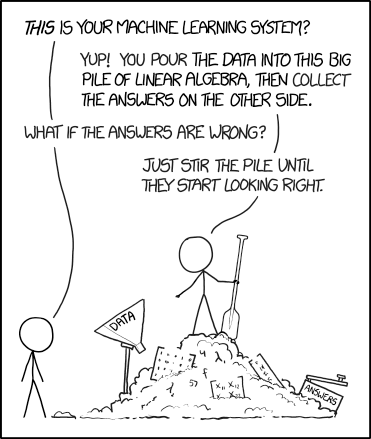
\includegraphics{images/machine-learning-xkcd.png}
\caption{Guy on a pile of data explaining how math and data have to be
stirred in a machine learning system until the right answers show up.
Credits: xkcd.com}
\end{figure}

\section{What to expect from this
book}\label{what-to-expect-from-this-book}

The book will teach you how to make (supervised) machine learning models
interpretable. It contains one or the other mathematical formula, but
it's kept at a manageable level of math. This book is not for people who
are trying to learn machine learning from scratch. If you are new to
machine learning, there are loads of books and other resources for
learning the basics. I recommend the book
\href{https://web.stanford.edu/~hastie/ElemStatLearn/}{Elements of
Statistical Learning} from \citet{Hastie2009} and
\href{https://www.coursera.org/learn/machine-learning}{Andrew Ng's
``Machine Learning'' online course on coursera} to get started with
machine learning. Both the book and the course are available for free!

This book starts out with exploring the concepts of machine learning
interpretability in Chapter \ref{interpretability}: It talks about when
interpretability is important and different types of explanations.
Definitions used throughout the book can be looked up in Chapter
\ref{definitions}. All models and methods are explained and demonstrated
with real data examples from Chapter \ref{data}. One way to make machine
learning interpretable is by using interpretable models, like linear
models or decision trees. Interpretable models are introduced in Chapter
\ref{simple}. The other option is to use model-agnostic interpretability
methods, which are the topic of Chapter \ref{agnostic}. This chapter
covers methods like partial dependence plots and permutation feature
importance. Model-agnostic methods work by changing the input of the
machine learning model and measuring changes in the output.

You can either read the book from start to end or directly jump to the
methods you are interested in. I hope you will enjoy the read!

\section{What is machine learning and why is it
important?}\label{what-is-machine-learning-and-why-is-it-important}

Machine learning is a method for teaching computers to make and improve
predictions or behaviours based on data.

Predicting the value of a house by learning from historical house sales
can be done with machine learning. The book focuses on supervised
machine learning, which includes all problems where we know the label or
the outcome of interest (e.g.~the past sale prices of houses) and want
to learn to predict. Excluded from supervised learning are, for example,
clustering tasks (=unsupervised learning), where we have no label, but
want to find clusters of data points. Also excluded are things like
reinforcement learning, where an agent learns to optimise some reward by
acting in an environment (e.g.~a computer playing Tetris). The goal in
supervised learning is to learn a predictive model that maps features
(e.g.~house size, location, type of floor, \ldots{}) to an output
(e.g.~value of the house). If the output is categorical, the task is
called classification and if it is numerical, then regression. Machine
learning is a set of algorithms that can learn these mappings from
training data, which are pairs of input features and a target. The
machine learning algorithm learns a model by changing parameters (like
linear weights) or learning structures (like trees). The algorithm is
guided by a score or loss function that is minimised. In the house value
example, the machine minimises some form of difference between the
estimated house sales price and the predicted sales price. A fully
trained machine learning model can then be used to make predictions for
new instances and be integrated into a product or process.

Estimating house values, recommending products, identifying street
signs, counting people on the street, assessing a person's credit
worthiness and detecting fraud: All these examples have in common that
they can and increasingly are realised with machine learning. The tasks
are different, but the approach is the same: Step 1 is to collect data.
The more, the better. The data needs to have the information you want to
predict and additional information from which the prediction should be
made. For a street sign detector (``Is there a street sign in the
image?'') you would collect street images and label them accordingly
with street sign yes vs.~no. For a loan default predictor you need
historical data from actual loans, the information if the customers
defaulted on their loans and data that helps you predict, like the
customers income, age and so on. For a house value estimator, you would
want to collect data from historical house sales and information about
the real estate like size, location and so on. Step 2: Feed this
information into a machine learning algorithm, which produces a sign
detector model, a credit worthiness model or a house value estimator.
This model can then be used in Step 3: Integrate the model into the
product or process, like a self-driving car, a loan application process
or a real estate marketplace website.

Machines exceed humans in a lot of tasks, like playing chess (or, since
recently, Go) or predicting the weather. Even if the machine is as good
as a human at a task, or slightly worse, there remain big advantages in
speed, reproducibility and scale. A machine learning model that has been
implemented once, can do a task much faster than humans, will reliably
produce the same results from the same input and can be copied
endlessly. Replicating a machine learning model on another machine is
fast and cheap. Training a second human to do a task can take decades
(especially when they are young) and is very costly. A big disadvantage
of using machine learning is that insights about the data and the task
the machine is solving are hidden within increasingly complex models.
You need millions of numbers to describe a deep neural network and there
is no way to understand the model in it's entirety. Other models, like
the RandomForest, consist of hundreds of decision trees that ``vote'' to
make predictions. Again, to fully understand how the decision was made,
you would need to look into the votes and structures of each of the
hundreds of trees. That just does not work out, no matter how clever you
are or how good your working memory is. The best performing models are
blends of multiple models (also called ensembles), which in itself
cannot be interpreted, even if each single model would be interpretable.
If you only focus on performance, you automatically will get more and
more opaque models. Just have a look at
\href{http://blog.kaggle.com/}{interviews with winners on the kaggle.com
machine learning competition platform}: The winning models were mostly
ensembles of models or very complex models like boosted trees or deep
neural networks.

\chapter{Interpretability}\label{interpretability}

So far, I haven't found a good scientific definition of ``Machine
learning model interpretability'' or how to measure the goodness of an
explanation. Throughout the book, I will use this rather simple, yet
elegant definition from \citet{miller2017explanation}:
\textbf{Interpretability is the degree to which a human can understand
the cause of a decision.} The higher the interpretability of a model,
the easier it is for someone to comprehend why certain decisions (read:
predictions) were made. A model has better interpretability than another
model, if it's decisions are easier to comprehend for a human than
decisions from the second model. I will be using both the terms
interpretable and explainable equally.

\section{The importance of machine learning
interpretability}\label{interpretability.importance}

If a machine learning model performs well, \textbf{why not just trust}
it and ignore why it made a certain decision?

Let's dive deeper into the reasons why interpretability is so important.
Machine learning has come to a state where you have to make a trade-off:
Do you simply want to know \textbf{what} is predicted happen? For
example if a client will churn or if a medication will work well for a
patient. Or do you want to know \textbf{why} something is predicted to
happen and paying for the interpretability with accuracy? In some cases
you don't care why a decision was made, only the assurance that the
predictive performance was good on a test dataset is enough. But in
other cases knowing the `why' can help you understand more about the
problem, the data and it can also tell you why a model might fail. Some
problems might not need explanations, because they either are low risk,
meaning a mistake has no severe consequences, (e.g.~a movie recommender
system) or the method has already been extensively studied and evaluated
(e.g.~optical character recognition). The necessity for interpretability
comes from an incompleteness in the problem formalisation
\citep{Doshi-Velez2017}, meaning that for certain problems or tasks it
is not enough to get the answer (the \textbf{what}), but the model also
has to give an explanation how it came to the answer (the \textbf{why}),
because correctly predicting is not enough to solve the problem.
Following reasons drive the demand for interpretability.

\begin{itemize}
\tightlist
\item
  There is a shift in many scientific disciplines from qualitative to
  quantitative methods (e.g.~sociology, psychology), and also towards
  machine learning (biology, genomics). The \textbf{goal of science} is
  to gain knowledge, but many problems can only be solved with big
  datasets and black box machine learning models. Interpretability
  allows to extract additional knowledge.
\item
  It is \textbf{human nature} wanting to understand things and to have
  some form of control.
\item
  Machine learning models are taking over real world tasks, that demand
  \textbf{safety measurements} and testing. A self-driving car
  automatically detects cyclists, which is as desired. You want to bet
  100\% sure that the abstraction the system learned will be fail-safe,
  because running over cyclists is quite bad. An explanation might
  reveal that the most important feature learned is to recognise the two
  wheels of a bike and this explanation helps to think about edge cases
  like bikes with side bags, that partially cover the wheels.
\item
  By default most machine learning models pick up biases from the
  training data. This can turn your machine learning models into racists
  which discriminate against protected groups. Interpretability is a
  useful debugging tool to \textbf{detect bias} in machine learning
  models.
\end{itemize}

Even in low risk environments, like movie recommendation,
interpretability in the research and development stage is valuable. Also
later when some model is used in a product, things can go wrong. And
need for interpretability arises when your model fucks up. Because
having an explanation for a faulty classification helps to understand
the cause of the fault. It delivers a direction for how to fix the
system. Consider an example of a husky versus wolf classifier, that
misclassifies some huskies as wolfs. If there is an explanation to the
classification you can see, that the misclassification happened due to
the snow on the image. The classifier learned to use snow as a feature
for classifying images as wolfs, which might make sense in terms of
separating features in the training data set, but not in the real world
use.

If you can ensure that the machine learning model can explain decisions,
following traits can also be checked more easily
\citep{Doshi-Velez2017}.

\begin{itemize}
\tightlist
\item
  Fairness: Unbiased, not discriminating against protected groups
  (implicit or explicit). An interpretable model can tell you why it
  decided a certain person is not worthy of a credit and for a human it
  becomes easy to decide if the decision was based on a learned
  demographic (e.g.~racial) bias.
\item
  Privacy: Sensitive information in the data is protected.
\item
  Reliability or Robustness: Small changes in the input don't lead to
  big changes in the prediction.
\item
  Causality: Only causal relationships are picked up. Meaning a
  predicted change in a decision due to arbitrary changes in the input
  values are also happening in reality.
\item
  Trust: It is easier for humans to trust into a system that explains
  it's decisions compared to a black box
\end{itemize}

\section{Scope of interpretability}\label{scope-of-interpretability}

An algorithm trains a model, which produces the predictions. Each step
can be evaluated in terms of transparency or interpretability.

\subsection{Algorithm transparency}\label{algorithm-transparency}

\emph{How does the algorithm create the model?}

Algorithm transparency is about how the algorithm learns a model from
the data and what kind of relationships it is capable of picking up. If
you are using convolutional neural networks for classifying images, you
can explain that the algorithm learns edge detectors and filters on the
lowest layers. This is an understanding of how the algorithm works, but
not of the specific model that is learned in the end and not about how
single predictions are made. For this level of transparency only
knowledge about the algorithm and not about the data or concrete learned
models are required. This book focuses on model interpretability and not
algorithm transparency. Algorithms like the least squares method for
linear models are well studied and understood. They score high in
transparency. Deep learning approaches (pushing a gradient through a
network with millions of weights) are less well understood and the inner
workings are in the focus of on-going research. It is not clear how they
exactly work, so they are less transparent.

\subsection{Global, holistic model
interpretability}\label{global-holistic-model-interpretability}

\emph{How does the trained model make predictions?}

You could call a model interpretable if you can comprehend the whole
model at once \citep{Lipton2016}. To explain the global model output,
you need the trained model, knowledge about the algorithm and the data.
This level of interpretability is about understanding how the model
makes the decisions, based on a holistic view on it's features and each
learned components like weights, parameters and structures. Which
features are the important ones and what kind of interactions are
happening? Global model interpretability helps to understand the
distribution of your target variable based on the features. Arguably,
global model interpretability is very hard to achieve in practice. Any
model that exceeds a handful of parameters or weights, probably won't
fit an average human's brain short term memory. I'd argue that you
cannot really imagine a linear model with 5 features and draw in your
head the hyperplane that was estimated in the 5-dimensional feature
space. Each feature space with more than 3 dimensions is just not
imaginable for humans. Usually when people try to comprehend a model,
they look at parts of it, like the weights in linear models.

\subsection{Global model interpretability on a modular
level}\label{global-model-interpretability-on-a-modular-level}

\emph{How do parts of the model influence predictions?}

You might not be able to comprehend a Naive Bayes model with many
hundred features, because there is no way you could hold all the feature
weights in your brain's working memory. But you can understand a single
weight easily. Not many models are interpretable on a strict parameter
level. While global model interpretability is usually out of reach,
there is a better chance to understand at least some models on a modular
level. In the case of linear models, the interpretable parts are the
weights and the distribution of the features, for trees it would be
splits (used feature plus the cut-off point) and leaf node predictions.
Linear models for example look like they would be perfectly
interpretable on a modular level, but the interpretation of a single
weight is interlocked with all of the other weights. As you will see in
Chapter \ref{limo}, the interpretation of a single weight always comes
with the footnote that the other input features stay at the same value,
which is not the case in many real world applications. A linear model
predicting the value of a house, which takes into account both the size
of the house and the number of rooms might have a negative weight for
the rooms feature, which is counter intuitive. But it can happen,
because there is already the highly correlated flat size feature and in
a market where people prefer bigger rooms, a flat with less rooms might
be worth less than a flat with more rooms when both have the same size.
The weights only make sense in the context of the other features used in
the model. But arguably the weights in a linear model still have better
interpretability than the weights of a deep neural network.

\subsection{Explain the prediction for a single
instance}\label{explain-the-prediction-for-a-single-instance}

\emph{Why did the model make a specific decision for an instance?}

You can zoom in on a single instance and examine what kind of prediction
the model makes for this input, and why it made this decision. When you
look at one example, the local distribution of the target variable might
behave more nicely. Locally it might depend only linearly or monotonic
on some features rather than having a complex dependence on the
features. For example the value of an apartment might not depend
linearly on the size, but if you only look at a specific apartment of
100 square meters and check how the prize changes going up plus and
minus 10 square meters there is a chance that this subregion in your
data space is linear. Local explanations can be more accurate compared
to global explanations because of this. This book presents methods that
can make single predictions more interpretable in Chapter
\ref{agnostic}.

\subsection{Explain the predictions for a group of
instances}\label{explain-the-predictions-for-a-group-of-instances}

\emph{Why did the model make specific decisions for a group of
instances?}

The model predictions for multiple instances can be explained by either
using methods for global model interpretability (on a modular level) or
single instance explanations. The global methods can be applied by
taking the group of instances pretending it's the complete dataset and
using the global methods on this subset. The single explanation methods
can be used on each instance and listed or aggregated afterwards for the
whole group.

\section{Evaluating interpretability}\label{evaluating-interpretability}

There is no real consensus what interpretability in machine learning is.
Also it is not clear how to measure it. But there is some first research
on it and the attempt to formulate some approaches for the evaluation,
as described in the following section.

\subsection{Approaches for evaluating the explanation
quality}\label{approaches-for-evaluating-the-explanation-quality}

\citet{Doshi-Velez2017} propose three major levels of evaluating
explainability.

\begin{itemize}
\tightlist
\item
  \textbf{Application level evaluation (real task)}: Put the explanation
  into the product and let the end user test it. For example, on an
  application level, radiologists would test fracture detection software
  (which includes a machine learning component to suggest where
  fractures might be in an x-ray image) directly in order to evaluate
  the model. This requires a good experimental setup and an idea of how
  to assess the quality. A good baseline for this is always how good a
  human would be at explaining the same decision.
\item
  \textbf{Human level evaluation (simple task)} is a simplified
  application level evaluation. The difference is that these experiments
  are not conducted with the domain experts, but with lay humans. This
  makes experiments less expensive (especially when the domain experts
  are radiologists) and it is easier to find more humans. An example
  would be to show a user different explanations and the human would
  choose the best.
\item
  \textbf{Function level evaluation (proxy task)} does not require any
  humans. This works best when the class of models used is already
  evaluated by someone else in a human level evaluation. For example it
  might be known that the end users understand decision trees. In this
  case, a proxy for explanation quality might be the depth of the tree.
  Shorter trees would get a better explainability rating. It would make
  sense to add the constraint that the predictive performance of the
  tree remains good and does not drop too much compared to a larger
  tree.
\end{itemize}

\subsubsection{More on function level
evaluation}\label{more-on-function-level-evaluation}

Model size is an easy way to measure explanation quality, but it is too
simplistic. For example, a sparse model with features that are
themselves not interpretable is still not a good explanation.

There are more dimensions to interpretability:

\begin{itemize}
\tightlist
\item
  Model sparsity: How many features are being used by the explanation?
\item
  Monotonicity: Is there a monotonicity constraint? Monotonicity means
  that a feature has a monotonic relationship with the target. If the
  feature increases, the target either always increases or always
  decreases, but never switches between increasing and decreasing.
\item
  Uncertainty: Is a measurement of uncertainty part of the explanation?
\item
  Interactions: Is the explanation able to include interactions of
  features?
\item
  Cognitive processing time: How long does it take to understand the
  explanation?
\item
  Feature complexity: What features were used for the explanation? PCA
  components are harder to understand than word occurrences, for
  example.
\item
  Description length of explanation
\end{itemize}

\chapter{Datasets}\label{data}

Throughout the book all the models and techniques will be applied on
real datasets, which are freely available online. We will be using
different datasets for different tasks: classification, regression and
text classification.

\section{Bike sharing counts (regression)}\label{bike-data}

This dataset contains daily counts of bike rentals from bike sharing
company \href{https://www.capitalbikeshare.com/}{Capital-Bikeshare} in
Washington D.C., along with weather and seasonal information. The data
was kindly open sourced by Capital-Bikeshare and the folks from
\citet{bike2013} have added the weather data and the seasonal
information. The goal is to predict how many rental bike will be out on
the street given weather and day. The data can be downloaded from the
\href{http://archive.ics.uci.edu/ml/datasets/Bike+Sharing+Dataset}{UCI
Machine Learning Repository}.

For the examples, new features were introduced and not all original
features used. Here is the list of features that were used:

\begin{itemize}
\tightlist
\item
  season : sprint (1), summer (2), autumn (3), winter (4)
\item
  holiday : Binary feature indicating if the day was a holiday (1) or
  not (0)
\item
  yr: The year (2011 or 2012)
\item
  days\_since\_2011: Number of days since the 01.01.2011 (the first day
  in the dataset). This feature was introduced to account for the trend,
  in this case that the bike rental service became more popular over
  time.
\item
  workingday : Binary feature indicating if the day was a workingday (1)
  or weekend / holiday (0).
\item
  weathersit : The weather situation on that day.

  \begin{itemize}
  \tightlist
  \item
    Clear, Few clouds, Partly cloudy, Partly cloudy
  \item
    Mist + Cloudy, Mist + Broken clouds, Mist + Few clouds, Mist
  \item
    Light Snow, Light Rain + Thunderstorm + Scattered clouds, Light Rain
    + Scattered clouds
  \item
    Heavy Rain + Ice Pallets + Thunderstorm + Mist, Snow + Fog
  \end{itemize}
\item
  temp : Temperature in Celsius
\item
  hum: Relative humidity in percent (0 to 100)
\item
  windspeed: Wind speed in km per hour
\item
  cnt: Count of total rental bikes including both casual and registered.
  The count was used as the target in the regression tasks.
\end{itemize}

\section{Youtube spam comments (text classification)}\label{spam-data}

As an example for text classification we will be using 1956 comments
from 5 different YouTube videos. Thankfully the authors that used this
dataset in an article about spam classification made the data
\href{http://dcomp.sor.ufscar.br/talmeida/youtubespamcollection/}{freely
available} \citep{alberto2015tubespam}.

The comments were collected through the YouTube API from five of the ten
most viewed videos on YouTube in the first half of 2015. All of the 5
videos are music videos. One of them is ``Gangnam Style'' from Korean
artist Psy. The other artists where Katy Perry, LMFAO, Eminem and
Shakira.

You can flip through some the comments. The comments had been hand
labeled as spam or legitimate. Spam has been coded with a `1' and
legitimate comments with a `0'.

\begin{tabular}{l|l|r}
\hline
  & CONTENT & CLASS\\
\hline
3 & just for test I have to say murdev.com & 1\\
\hline
4 & me shaking my sexy ass on my channel enjoy \textasciicircum{}\_\textasciicircum{} & 1\\
\hline
5 & watch?v=vtaRGgvGtWQ   Check this out . & 1\\
\hline
6 & Hey, check out my new website!! This site is about kids stuff. kidsmediausa  . com & 1\\
\hline
7 & Subscribe to my channel & 1\\
\hline
8 & i turned it on mute as soon is i came on i just wanted to check the  views... & 0\\
\hline
9 & You should check my channel for Funny VIDEOS!! & 1\\
\hline
10 & and u should.d check my channel and tell me what I should do next! & 1\\
\hline
11 & Hey subscribe to me & 1\\
\hline
\end{tabular}

You could also go over to YouTube and have a look at the comment
section. But please don't get trapped in the YouTube hell, ending up
watching videos about monkeys stealing and drinking coktails from
tourists on the beach. Also the Google Spam detector probably has
changed a lot since 2015.

\section{Risk factors for cervical cancer
(classification)}\label{cervical-data}

The cervical cancer dataset contains indicators and risk factors for
predicting if a woman will get cervical cancer. The features contain
demographics (e.g.~age), habits and medical history. The data can be
downloaded from the
\href{https://archive.ics.uci.edu/ml/datasets/Cervical+cancer+\%28Risk+Factors\%29}{UCI
Machine Learning repository} is described by
\citet{fernandes2017transfer}.

The subset of features, which are used in this book are:

\begin{itemize}
\tightlist
\item
  (int) Age
\item
  (int) Number of sexual partners
\item
  (int) First sexual intercourse (age)
\item
  (int) Num of pregnancies
\item
  (bool) Smokes yes (1) or no (1)
\item
  (int) Smokes (years)
\item
  (bool) Hormonal Contraceptives yes (1) vs no (0)
\item
  (int) Hormonal Contraceptives (years)
\item
  (bool) IUD: Intrauterine device yes (1) vs no (1)
\item
  (int) IUD (years): Number of years with an intrauterine device
\item
  (bool) STDs: Ever had a sexually transmitted disease? Yes (1) vs no
  (0)
\item
  (int) STDs (number): Number of sexually transmitted diseases.
\item
  (int) STDs: Number of diagnosis
\item
  (int) STDs: Time since first diagnosis
\item
  (int) STDs: Time since last diagnosis
\item
  (bool) Biopsy: Biopsy results ``Healthy'' or ``Cancer''. Target
  outcome.
\end{itemize}

As the biopsy serves as the gold standard for diagnosing cervical
cancer, the classification task in this book used the biopsy outcome as
the target. Missing values for each column were imputed by the mode
(most frequent value), which is probably a bad solution, because the
value of the answer might be correlated with the probability for
missingness. There is probably a bias, because the question are of a
very private nature. But this is not a book about missing data
imputation, so the mode imputation will suffice!

\chapter{Definitions}\label{definitions}

To avoid confusion through ambiguity, here are some definitions of terms
used in this book.

\begin{itemize}
\tightlist
\item
  An \textbf{Algorithm} is a set of rules that a machine follows to
  achieve a particular goal \citep{algorithm}
\item
  A \textbf{Machine learning algorithm} is a set of rules that a machine
  follows to learn how to a achieve a particular goal. The output of a
  machine learning algorithm is a machine learning model.
\item
  A \textbf{(Machine learning) Model} is the outcome of a machine
  learning algorithm. This can be a set of weights for a linear model or
  neural network plus the information about the architecture.
\item
  \textbf{Dataset}: A table containing the data from which the machine
  learns.
\item
  \textbf{Features}: The features/information used for
  prediction/classification/clustering. A feature is one column in the
  dataset.
\item
  \textbf{Target}: The thing the machine learns to predict.
\item
  \textbf{(machine learning) Task}: The combination of a dataset with
  features and a target. Depending on the type of the target, the task
  can be classification, regression, survival analysis, clustering or
  outlier detection.
\item
  \textbf{Prediction}: The machine learning models ``guess'' what the
  target's value should be based on the given features.
\item
  \textbf{Instance}: One row in the dataset.
\end{itemize}

\chapter{Interpretable models}\label{simple}

The most straightforward way to get to interpretable machine learning is
to use only a subset of algorithms that create interpretable models.

Very common model types of this group of interpretable models are:

\begin{itemize}
\tightlist
\item
  Linear regression model
\item
  Logistic regression
\item
  Decision trees
\end{itemize}

In the following chapters we will talk about these models. Not in
detail, only the basics, because there are already a ton of books,
videos, tutorials, papers and more material. We will focus on how to
interpret the models. The chapter covers linear models, logistic
regression and decision trees in details and lists some more.

All of the interpretable models types explained in this book are
interpretable on a modular level, except for the k-nearest neighbours
method. The following table gives an overview over the interpretable
model types and their properties. A model is linear if the association
between features and target is modelled linearly. A monotonic model
ensures that the relationship between a feature and the target outcome
is always in the same direction over the whole range of the feature: an
increase in the features value will consistently lead to either an
increase or a decrease of the target outcome, but never both for this
feature. Monotonicity is useful for the interpretation of a model,
because it makes it easier to understand a relationship. Some models can
automatically include interactions between the features for predicting
the outcome. You can always include interactions into any kind of model
by manually creating interaction features. This can be important for
correctly predicting the outcome, but too many or too complex
interactions can hurt interpretability. Some models only handle
regression, some only classification and some can manage to do both.

You can use this table to choose a suitable interpretable model for your
task.

\begin{longtable}[]{@{}lllll@{}}
\toprule
Algorithm & Linear & Monotonicity & Interactions & Task
type\tabularnewline
\midrule
\endhead
Linear models & Yes & Yes & No & Regression\tabularnewline
Logistic regression & No & Yes & No & Classification\tabularnewline
Decision trees & No & No & Yes & Class. + Regr.\tabularnewline
Naive Bayes & Yes & Yes & No & Classification\tabularnewline
k-nearest neighbours & No & No & No & Class. + Regr.\tabularnewline
RuleFit & Partially & No & Yes & Class. + Regr.\tabularnewline
\bottomrule
\end{longtable}

\section{Terminology}\label{terminology}

\begin{itemize}
\tightlist
\item
  Y is the target outcome.
\item
  X are the features (also called variables, covariables, covariates or
  inputs).
\item
  \(\beta\) are regression weights (also called coefficients).
\end{itemize}

\section{Linear models}\label{limo}

Linear models have been used since a long time by statisticians,
computer scientists and other people with quantitative problems. Linear
models learn linear (and therefore monotonic) relationships between the
features and the target. The linearity of the learned relationship makes
the interpretation easy.

Linear models can be used to model the dependency of a regression target
\(y\) on \(p\) features \(x\). The learned relationships are linear and,
for a singular instance \(i\), can be written as:

\[y_{i} = \beta_{0} + \beta_{1} \cdot x_{i1} + \ldots + \beta_{p} x_{ip} + \epsilon_{i}\]

The i-th instance's outcome is a weighted sum of it's \(p\) features.
The \(\beta_{j}\) represent the learned feature weights or coefficients.
The \(\epsilon_{i}\) is the error we are still making, the difference
between the predicted and actual outcome.

Different methods can be used to estimate the optimal weight vector
\(\mathbf{\hat{\beta}}\). The ordinary least squares method is commonly
used to find the weights that minimise the squared difference between
the actual and the estimated outcome:
\[\mathbf{\hat{\beta}} = \arg\!\min_{\beta_0, \ldots, \beta_p} \sum_{i=1}^n \left(y_i - \left(\beta_0 + \sum_{j=1}^p \beta_j x_{ij}\right)\right)\]

We won't go into detail about how the optimal weights can be found, but
if you are interested you can read Chapter 3.2 of the book ``Elements of
Statistical Learning'' \citep{Hastie2009} or one of the other zillions
of sources about linear regression models.

The biggest advantage of linear regression models is the linearity: It
makes the estimation procedure straightforward and most importantly
these linear equations have an easy to understand interpretation on a
modular level (i.e.~the weights). That is one of the main reasons why
the linear model and all similar models are so widespread in academic
fields like medicine, sociology, psychology and many more quantitative
research fields. In this areas it is important to not only predict
e.g.~the clinical outcome of a patient, but also to quantify the
influence of the medication while at the same time accounting for things
like sex, age and other features in an interpretable manner.

Linear regression models also come with some assumptions that make them
easy to use and interpret but which are often not satisfied in reality.
Assumed is: Linearity, normality, homoscedasticity, independence, fixed
features and absence of multicollinearity.

\begin{itemize}
\tightlist
\item
  \textbf{Linearity}: Linear regression models force the estimated
  response to be a linear combination of the features, which is both the
  greatest strength and biggest limitation. Linearity leads to
  interpretable models: linear effects are simple to quantify and
  describe (see also next chapter) and are additive, so it is easy to
  separate the effects. If you suspect interactions of features or a
  non-linear association of a feature with the target value, then you
  can add interaction terms and use techniques like regression splines
  to estimate non-linear effects.
\item
  \textbf{Normality}: The target outcome given the features are assumed
  to follow a normal distribution. If this assumption is violated, then
  the estimated confidence intervals of the feature weights are not
  valid. Any interpretation of the features p-values is not valid.
\item
  \textbf{Homoscedasticity} (constant variance): The variance of the
  error terms \(\epsilon_{i}\) is assumed to be constant over the whole
  feature space. Let's say you want to predict the value of a house
  given the living area in square meters. You estimate a linear model,
  which assumes that no matter how big the flat, the error terms around
  the predicted response have the same variance. This assumption is
  often violated in reality. In the house example it is plausible that
  the variance of error terms around the predicted price is higher for
  bigger houses, since also the prices are higher and there is more room
  for prices to vary.
\item
  \textbf{Independence}: Each instance is assumed to be independent from
  the next one. If you have repeated measurements, like multiple records
  per patient, the data points are not independent from each other and
  there are special linear model classes to deal with these cases, like
  mixed effect models or GEEs.
\item
  \textbf{Fixed features}: The input features are seen as `fixed',
  carrying no errors or variation, which, of course, is very unrealistic
  and only makes sense in controlled experimental settings. But not
  assuming fixed features would mean that you have to fit very complex
  measurement error models that account for the measurement errors of
  your input features. And usually you don't want to do that.
\item
  \textbf{Absence of multicollinearity}: Basically you don't want
  features to be highly correlated, because this messes up the
  estimation of the weights. In a situation where two features are
  highly correlated (something like correlation \textgreater{} 0.9) it
  will become problematic to estimate the weights, since the feature
  effects are additive and it becomes indeterminable to which of the
  correlated features to attribute the effects.
\end{itemize}

\subsection{Interpretation}\label{interpretation}

The interpretation of a weights in the linear model depends on the type
of the corresponding feature:

\begin{itemize}
\tightlist
\item
  Numerical feature: For an increase of the numerical feature \(x_{j}\)
  by one point, the estimated outcome changes by \(\beta_{j}\). An
  example for a numerical feature is the size of a house.
\item
  Binary feature: A feature, that for each instance takes on one of two
  possible values. An example is the feature ``House comes with a
  garden''. One of the values counts as the reference level (in some
  programming languages coded with 0), like ``No garden''. A change of
  the feature \(x_{j}\) from the reference level to the other level
  changes the estimated outcome by \(\beta_{j}\)
\item
  Categorical feature with multiple levels: A feature with a fixed
  amount of possible values. An example is the feature ``Floor type'',
  with possible levels ``carpet'', ``laminate'' and ``parquet''. One
  solution to deal with many levels is to one-hot-encode them, meaning
  each level gets it's own column. From a categorical feature with \(l\)
  levels, you only need \(l-1\) columns, otherwise the coding is
  overparameterised. The interpretation for each level is then according
  to the binary features. Some language like R allow you to code
  categorical feature in different ways, see Chapter @ref(cat.code)
\item
  Intercept \(\beta_{0}\): The intercept is the feature weight for the
  constant feature, which is always 1 for all instances. Most software
  packages automatically add this feature for estimating the intercept.
  The interpretation is: Given all numerical features are zero and the
  categorical features are at the reference level, the estimated outcome
  of \(y_{i}\) is \(\beta_{0}\). The interpretation of \(\beta_{0}\) is
  usually not relevant, because instances with all features at zero
  often don't make any sense, unless the features were standardised
  (mean of zero, standard deviation of one), where the intercept
  \(\beta_0\) reflects the predicted outcome of an instance where all
  features are at their mean.
\end{itemize}

Another important measurement for interpreting linear models is the
\(R^2\) measurement. \(R^2\) tells you how much of the total variance of
your target outcome is explained by the model. The higher \(R^2\) the
better your model explains the data. The formula to calculate \(R^2\)
is: \(R^2 = 1 - SSE/SST\), where SSE is the squared sum of the error
terms (\(SSE = \sum_{i=1}^n (y_i - \hat{y}_i)^2\)) and SST is the
squared sum of the data variance
(\(SST = \sum_{i=1}^n (y_i - \bar{y})^2\)). The SSE tells you how much
variance remains after fitting the linear model, which is measured by
looking at the squared differences between the predicted and actual
target values. SST is the total variance of the target around the mean.
So \(R^2\) tells you how much of your variance can be explained by the
linear model. \(R^2\) ranges between 0 for models that explain nothing
and 1 for models that explain all of the variance in your data.

There is a catch, because \(R^2\) increases with the number of features
in the model, even if they carry no information about the target value
at all. So it is better to use the adjusted R-squared (\(\bar{R}^2\)),
which accounts for the number of features used in the model. It's
calculation is \(\bar{R}^2 = R^2 - (1-R^2)\frac{p}{n - p - 1}\), where
\(p\) is the number of features and \(n\) the number of instances.

It isn't helpful to do interpretation on a model with very low \(R^2\)
or \(\bar{R}^2\), because basically the model is not explaining much of
the variance, so any interpretation of the weights are not meaningful.

\subsection{Interpretation example}\label{interpretation-example}

In this example we use the linear model to predict the bike rentals on a
day, given weather and calendrical information, see Chapter
\ref{bike-data}. For the interpretation we examine the estimated
regression weights. The features are a mix of numerical and categorical
features.

\begin{tabular}{l|r|r}
\hline
  & Estimate & Std. Error\\
\hline
(Intercept) & 2579.8 & 251.6\\
\hline
seasonSUMMER & 864.8 & 131.0\\
\hline
seasonFALL & 54.3 & 175.0\\
\hline
seasonWINTER & 319.6 & 119.4\\
\hline
holidayHOLIDAY & -639.8 & 217.2\\
\hline
workingdayWORKING DAY & 67.2 & 78.2\\
\hline
weathersitMISTY & -394.5 & 94.3\\
\hline
weathersitRAIN/SNOW/STORM & -1863.5 & 225.0\\
\hline
temp & 109.0 & 7.6\\
\hline
hum & -18.0 & 3.3\\
\hline
windspeed & -45.3 & 7.3\\
\hline
days\_since\_2011 & 5.0 & 0.2\\
\hline
\end{tabular}

Interpretation of a numerical feature (`Temperature'): An increase of
the temperature by 1 degree Celsius increases the expected number of
bikes by 109.0 given all other features stay the same.

Interpretation of a categorical feature (`weathersituation')): The
estimated number of bikes is -1863.5 lower when it is rainy, snowing or
stormy, compared to good weather, given that all features stay the same.
Also if the weather was misty, the expected number of bike rentals was
-394.5 lower, compared to good weather, given all other features stay
the same.

As you can see in the interpretation examples, the interpretations
always come with the footnote that `all other features stay the same'.
That's because of the nature of linear models: The target is a linear
combination of the weighted features. The estimated linear equation
spans a hyperplane in the feature/target space (a simple line in the
case of a single feature). The \(\beta\)'s specify the slope (gradient)
of the hyperplane in each direction. The good side is, that it isolates
the interpretation. If you think of the features as turn-switches that
you can turn up or down, it is nice to see what happens when you would
just turn the switch for one feature. On the bad side of things, the
interpretation ignores the joint distribution with other features.
Increasing one feature, but not changing others, might create
unrealistic or at least unlikely data points.

\subsection{Interpretation templates}\label{interpretation-templates}

The interpretation of the features in the linear model can be automated
by using following text templates.

\textbf{Interpretation of a numerical feature}

An increase of \(x_{k}\) by one unit increases the expectation for \(y\)
by \(\beta_k\) units, given all other features stay the same.

\textbf{Interpretation of a categorical feature}

A change from \(x_{k}\)'s reference level to the other category
increases the expectation for \(y\) by \(\beta_{k}\), given all other
features stay the same.

\subsection{Visual parameter
interpretation}\label{visual-parameter-interpretation}

Different visualisations make the linear model outcomes easier and
quicker to grasp for humans.

\subsubsection{Weight plot}\label{weight-plot}

The information of the coefficient table (weight estimates and variance)
can be visualised. Figure \ref{fig:linear-weights-plot} shows a weight
plot of the linear model fitted before.

\textbackslash{}begin\{figure\}

\{\centering 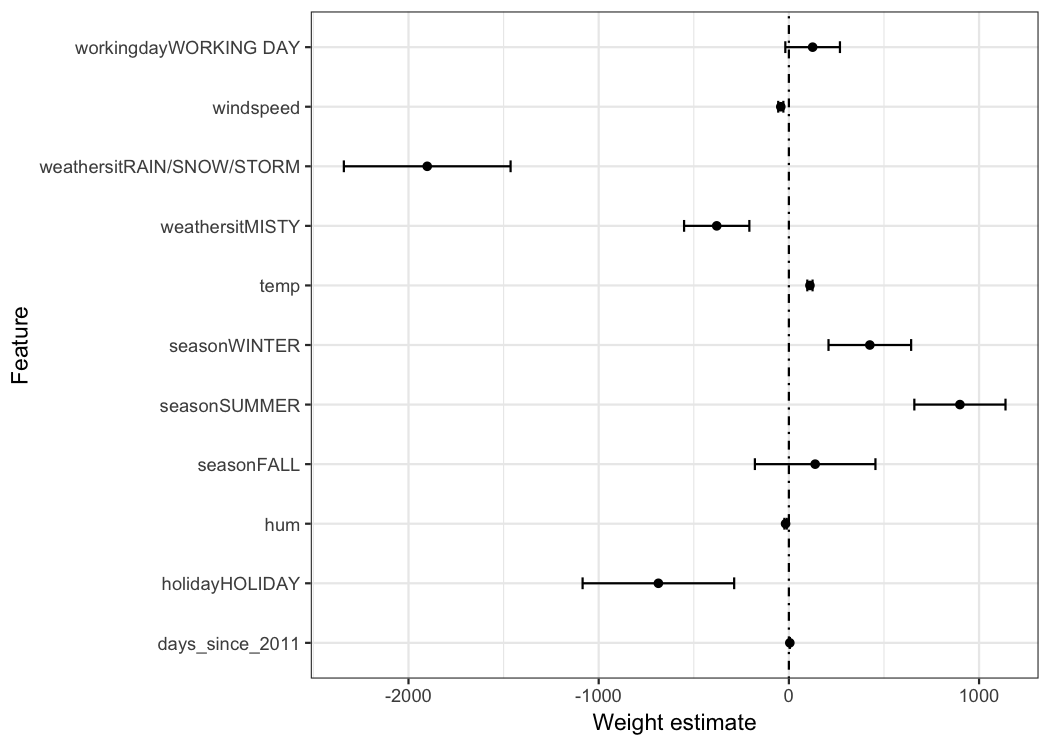
\includegraphics{xai-book_files/figure-latex/linear-weights-plot-1}

\}

\textbackslash{}caption\{Each row in the plot represents one feature
weight. The weights are displayed as points and the 95\% confidence
intervals around the points with a line. A 95\% confidence interval
means that if the linear model would be estimated 100 times on similar
data, in 95 out of 100 times, the confidence interval would cover the
true weight, under the linear model assumptions (linearity, normality,
homoscedasticity, independence, fixed features, absence of
multicollinearity).\}\label{fig:linear-weights-plot}
\textbackslash{}end\{figure\} Figure \ref{fig:linear-weights-plot} makes
clear that rainy/snowy/stormy weather has a strong negative effect on
the expected number of bikes. The working day feature's weight is close
to zero and the zero is included in the 95\% interval, meaning it is not
influencing the prediction significantly. Some confidence intervals are
very short and the estimates are close to zero, yet the features were
important. Temperature is such a candidate. The problem about the weight
plot is that the features are measured on different scales. While for
weather situation feature the estimated \(\beta\) signifies the
difference between good and rainy/storm/snowy weather, for temperature
it signifies only an increase of 1 degree Celsius. You can improve the
comparison by scaling the features to mean zero and standard deviation
of one before fitting the linear model, to make the estimated weights
comparable.

\subsubsection{Effect plot}\label{effect-plot}

The weights of the linear model can be analysed more meaningfully, when
multiplied with the actual feature values. The weights depend on the
scale of the features and will be different if you have a feature
measuring some height and you switch from meters to centimetres. The
weight will change, but the actual relationships in your data will not.
Also it is important to know the distribution of your feature in the
data, because if you have a very low variance, it means that almost all
instances will get a similar contribution from this feature. The effect
plot can help to understand how much the combination of a weight and a
feature contributes to the predictions in your data. Start with the
computation of the effects, which is the weight per feature times the
feature of an instance: \(\text{effect}_{i,j} = w_{j} \cdot x_{i,j}\).
The resulting effects are visualised with boxplots: A box in a boxplot
contains the effect range for half of your data (25\% to 75\% effect
quantiles). The line in the box is the median effect, so 50\% of the
instances have a lower and the other half a higher effect on the
prediction than the median value. The lines reach up to
\(+/- 1.58 \text{ IQR} / \sqrt{n}\), with IQR being the inter quartile
range (\(q_{0.75} - q_{0.25}\)). The points are outliers. The categorial
feature effects can be aggregated into one boxplot, compared to the
weight plot, where each weight gets a row.

\begin{figure}

{\centering 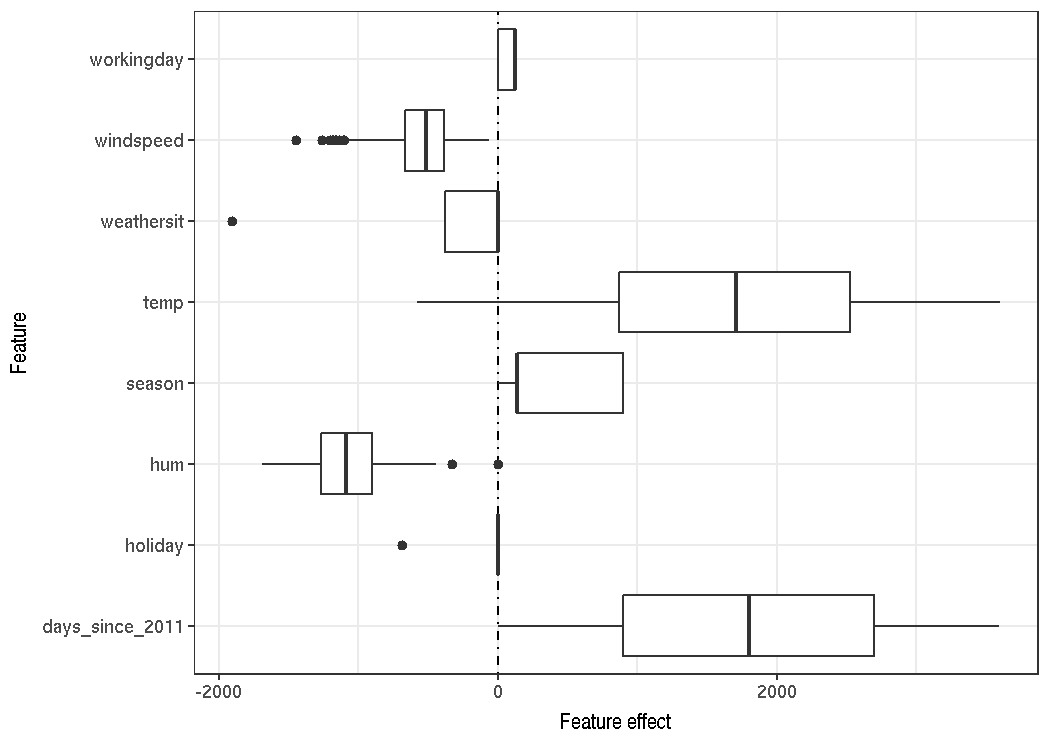
\includegraphics{xai-book_files/figure-latex/linear-effects-1} 

}

\caption{The feature effect plot shows the distribution of the effects (= feature value times feature weight) over the dataset for each feature.}\label{fig:linear-effects}
\end{figure}

The largest contributions to the expected number of bike rentals come
from temperature and the days feature, which captures the trend that the
bike rental service became more popular over time. The temperature has a
broad contribution distribution. The day trend feature goes from zero to
large positive contribution, because the first day in the dataset
(01.01.2011) get's a very low day effect, and the estimated weight with
this feature is positive (4.98), so the effect gets higher with every
day and is highest for the latest day in the dataset (31.12.2012). Note
that for effects from a feature with a negative weight, the instances
with a positive effect are the ones that have a negative feature value,
so days with a high negative effect of windspeed on the bike rental
count have the highest windspeeds.

\subsection{Explaining single
predictions}\label{explaining-single-predictions}

How much did each feature of an instance contribute towards the
prediction? This can, again, be answered by bringing together the
weights and feature values of this instance and computing the effects.
An interpretation of instance specific effects is only meaningful in
comparison with the distribution of each feature's effects.

\begin{figure}

{\centering 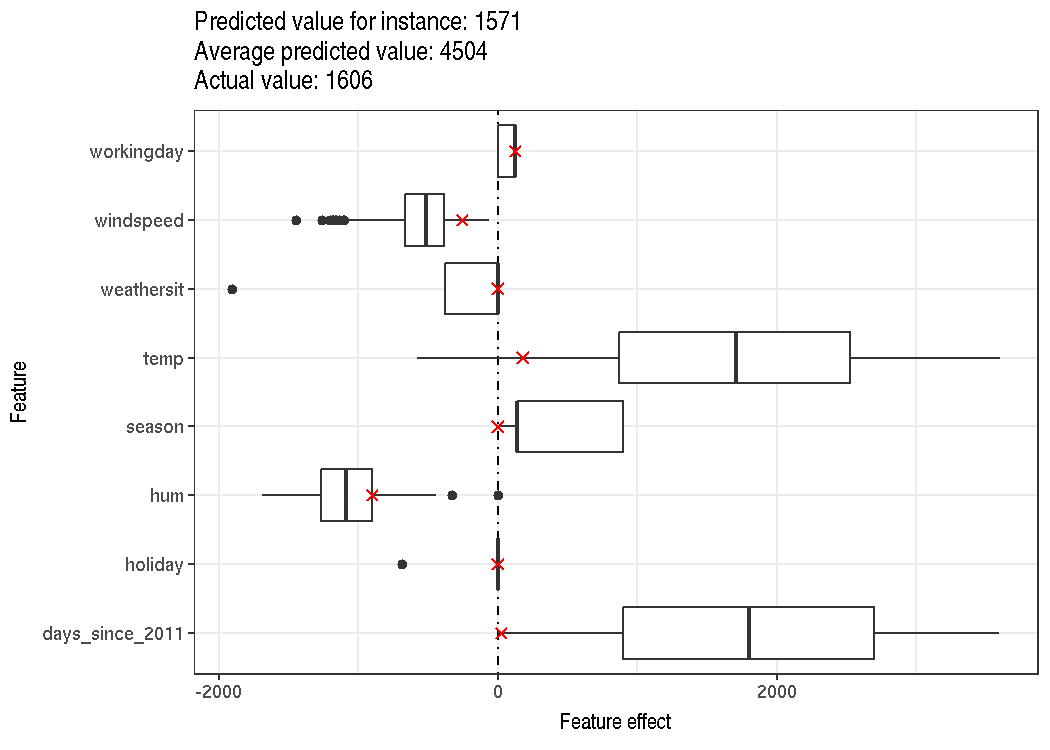
\includegraphics{xai-book_files/figure-latex/linear-effects-single-1} 

}

\caption{The effect for one instance shows the effect distribution while highlighting the effects of the instance of interest.}\label{fig:linear-effects-single}
\end{figure}

Let's have a look at the effect realisation for the rental bike count of
one instance (= one day). Some features contribute unusually little or
much to the predicted bike count, compared to the overall dataset:
Temperature (5 degrees) contributes less towards the predicted value
compared to the average and the trend feature ``days\_since\_2011''
unusually much, because this instance is from late 2011 (698 days).

\subsection{Coding categorical features}\label{cat.code}

There are several ways to encode a categorical feature and the choice
influences the interpretation of the \(\beta\)-weights.

Described in Chapter \ref{limo} is the treatment coding, which is
sufficient in most cases. Using different codings boils down to creating
different matrices (=design matrix) from your one column with the
categorical feature. This section presents three different codings, but
there are many more. The example used has six instances and one
categorical feature with 3 levels. For the first two instances, the
feature takes on category A, for instances three and four category B and
for the last two instances category C.

\begin{itemize}
\tightlist
\item
  \textbf{Treatment coding}: The \(\beta\) per level is the estimated
  difference in \(y\) compared to the reference level. The intercept of
  the linear model is the mean of the reference group (given all other
  features stay the same). The first column of the design matrix is the
  intercept, which is always 1. Column two is an indicator whether
  instance \(i\) is in category B, column three is an indicator for
  category C. There is no need for a column for category A, because then
  the linear equation would be overspecified and no unique solution (=
  unique \(\beta\)'s) can be found. Knowing that an instance is neither
  in category B or C is enough. \[
  \begin{pmatrix}
  1 & 0 & 0 \\
  1 & 0 & 0 \\
  1 & 1 & 0 \\
  1 & 1 & 0 \\
  1 & 0 & 1 \\
  1 & 0 & 1 \\
  \end{pmatrix}
  \]
\item
  \textbf{Effect coding}: The \(\beta\) per level is the estimated
  \(y\)-difference from the level to the overall mean (again, given all
  other features are zero or the reference level). The first column is
  again used to estimate the intercept. The weight \(\beta_{0}\) which
  is associated with the intercept represents the overall mean and
  \(\beta_{1}\), the weight for column two is the difference between the
  overall mean and category B. The overall effect of category B is
  \(\beta_{0} + \beta_{1}\). The interpretation for category C is
  equivalent. For the reference category A, \(-(\beta_{1} + \beta_{2})\)
  is the difference to the overall mean and
  \(\beta_{0} -(\beta_{1} + \beta_{2})\) the overall effect. \[
  \begin{pmatrix}
  1 & -1 & -1 \\
  1 & -1 & -1 \\
  1 & 1 & 0 \\
  1 & 1 & 0 \\
  1 & 0 & 1 \\
  1 & 0 & 1 \\
  \end{pmatrix}
  \]
\item
  \textbf{Dummy coding}: The \(\beta\) per level is the estimated mean
  of \(y\) for each level (given all feature are at value zero or
  reference level). Note that the intercept was dropped here, so that a
  unique solution for the linear model weights can be found. \[
  \begin{pmatrix}
  1 & 0 & 0 \\
  1 & 0 & 0 \\
  0 & 1 & 0 \\
  0 & 1 & 0 \\
  0 & 0 & 1 \\
  0 & 0 & 1 \\
  \end{pmatrix}
  \]
\end{itemize}

If you want to dive a bit deeper into different encodings of categorical
features, checkout
\href{http://stats.idre.ucla.edu/r/library/r-library-contrast-coding-systems-for-categorical-variables/}{this
webpage} and \href{http://heidiseibold.github.io/page7/}{this blog
post}.

\subsection{The disadvantages of linear
models}\label{the-disadvantages-of-linear-models}

They can only represent linear relationships as the name suggests. Each
non-linearity or interaction has to be hand-crafted and explicitly given
to the model as an input feature. Because of possible high correlation
between features, it is possible that a feature that is positively
correlated with the outcome might get a negative weight in a linear
model, because in the high dimensional space it is negatively
correlated. An example: You have a model to predict the rent price and
have features like number of rooms and size of the flat. Of course flat
size and room number are highly correlated, the bigger a flat the more
rooms it has. If you now take both features into a linear model it might
happen, that the flat size is the better predictor and get's a large
positive weight. The room number might end up getting a negative weight,
because given that a flat has the same size, increasing the number of
rooms could make it less valuable.

\subsection{Towards more complex relationships within linear model
class}\label{towards-more-complex-relationships-within-linear-model-class}

\begin{itemize}
\tightlist
\item
  Adding interactions
\item
  Adding non-linear terms like polynomials
\item
  Stratifying data by feature and fitting linear models on subsets
\end{itemize}

\section{Sparse linear models}\label{sparse-linear-models}

The examples for the linear models that I chose look all nice and tidy,
right? But in reality you might not have just a handful of features, but
hundreds or thousands. And your normal linear models? Interpretability
goes downriver. But there are ways to introduce sparsity (= only keeping
a few features) into the linear models. The most automatic and
convenient to use is the LASSO method. LASSO stands for ``least absolute
shrinkage and selection operator'' and when added to a linear model, it
performs feature selection and regularisation of the selected features.
We did not dive into the optimisation problem of finding the best
coefficients of the linear model. But basically it involves solving the
least-squares equation:
\[ min_{\beta_0,\beta} \left( \frac{1}{n} \sum_{i=1}^n (y_i - \beta_0 - x_i^T \beta)^2\right)\]
LASSO adds a term to this optimisation problem:
\[ min_{\beta_0,\beta} \left( \frac{1}{n} \sum_{i=1}^n (y_i - \beta_0 - x_i^T \beta)^2 + \lambda ||\beta||_1\right)\]
The term \(||\beta||_1\) is the L1-norm of the feature vector, that
leads to a penalisation of large values in \(\beta\). Since the L1-norm
is used, many of the coefficients for the features will get an estimate
of 0 and the others are shrunk. The weight \(\lambda\) says how strong
the regularising effect should be and is usually tuned by doing
cross-validation. Especially when \(\lambda\) is large, many
coefficients are driven to 0.

There are lots of other methods for reducing the number of features in
your linear regression model:

Methods that include a pre-processing step: - Hand selected features:
You can always use expert knowledge to choose and discard some features.
The big drawback is, that it can't be automated and you might not be an
expert. - Use some measure to pre-select features: An example is the
correlation coefficient. You only take features into account that exceed
some chosen threshold of correlation between the feature and the target.
Disadvantage is that it only looks at the features one at a time. Some
features might only show correlation after the linear model has
accounted for some other features. Those you will miss with this
approach.

Then there are also step-wise procedures: - Forward selection: Fit the
linear model with one feature. Do that with each feature. Choose the
model that works best (for example decided by R squared measurement).
Now again, for the remaining features, fit different versions of your
model by adding each feature. Pick the one that performs best again.
Continue until some criterium is reached, like the maximum number of
features in the model. - Backward selection: Same as forward selection,
but instead of adding features, start with the model with all features
and try which feature removal brings the best performance increase until
some stopping criterium is reached.

I recommend using LASSO. It also works for the logistic regression model
for classification models, which is the topic of the following chapter.

\section{Logistic regression: a linear model for
classification}\label{logistic-regression-a-linear-model-for-classification}

Logistic regression is the linear regression models counterpart for
classification problems.

\subsection{What's wrong with linear regression for
classification?}\label{whats-wrong-with-linear-regression-for-classification}

The gaussian linear model works well in most regression setup, but fails
in the classification case. Why is that? In case of two classes, you
could label one of the classes with 0 and the other with a 1 and use a
linear model on it and it would work. There are a few problems with that
approach:

\begin{itemize}
\tightlist
\item
  A linear model does try to give you probabilities, but it treats the
  classes as numbers (0 and 1) and fits the best hyperplane (if you have
  one feature, it's a line) that minimizes the distances between the
  points and the hyperplane. So it simply interpolates between the
  points, but there is no meaning in it and you cannot interpret it as
  probabilities.
\item
  Also a linear model will extrapolate the features and give you values
  below zero and above one, which are not meaningful and should tell you
  that there might be a more clever approach to doing classification.
\item
  Since the predicted outcome is not a probability but some linear
  interpolation between points there is no meaningful threshold at which
  you can distinguish one class from the other. A good illustration of
  this issue was given on
  (Stackoverflow){[}\url{https://stats.stackexchange.com/questions/22381/why-not-approach-classification-through-regression}{]},
  which I reproduced in Figure @ref\{fig:linear-class-threshold\}
\item
  Linear models don't extend to classification problems with multiple
  classes. You would have to start giving labeling the next class with a
  2, then 3 and so on. The classes might not have any order to them, but
  the linear model would force a weird structure on the relationship
  between the features and your class predictions. So for all features
  with a positive weight, the higher the features value the more they
  contribute to the prediction of a class with a higher number, even if
  the classes with similar numbers are not really related.
\end{itemize}

\begin{figure}
\centering
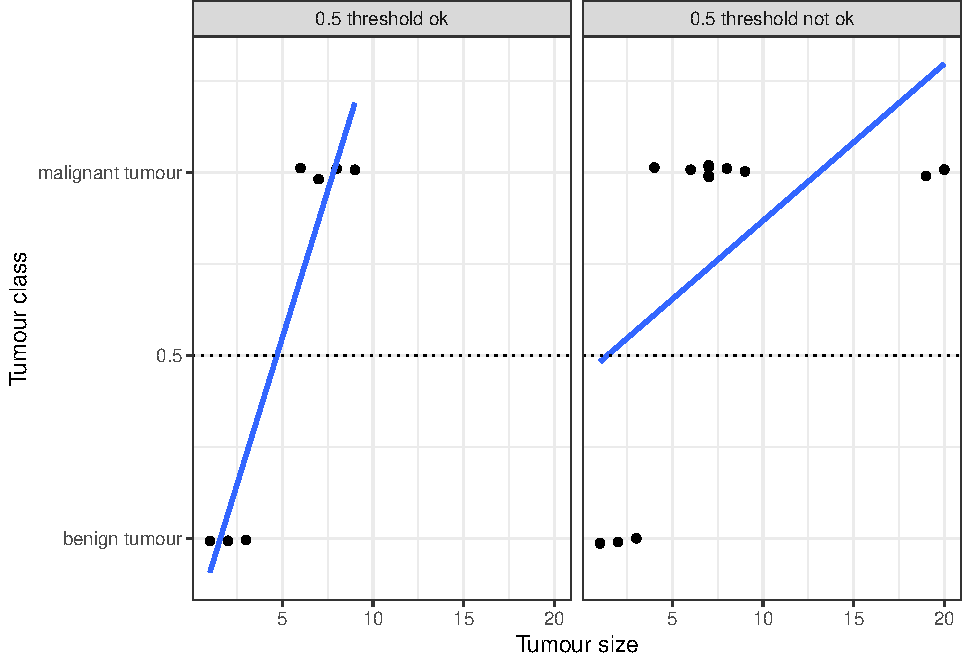
\includegraphics{xai-book_files/figure-latex/linear-class-threshold-1.pdf}
\caption{\label{fig:linear-class-threshold}An illustration why linear
regression does not work well in a binary classification setting. A
linear model is fitted on the artificial task of classifying a tumor as
malignant (1) or benign (0) depending on the tumor size. Each point is a
tumor, the x-axis shows the size of the tumor, the y-axis the
malignancy, points are slightly jittered to avoid overplotting of
points. The lines display the fitted curve from the linear model. In the
data setting on the left, we can use 0.5 as a threshold for the
predicted outcome of the linear model for seperating benign from
malignant tumors. After introducing a few more malignant tumor cases,
especially one with a large tumor size the regression line shifts and a
threshold of 0.5 would not separate the classes any longer. That's a
reason why logistic regression is better suited for classification
problems.}
\end{figure}

\subsection{Logistic regression}\label{logistic-regression}

The solution is logistic regression. Instead of fitting a straight
line/hyperplane and uses a non-linear function, the logistic function to
squeeze the output between 0 and 1. The logistic function is defined as
\[ logistic(\eta) = \frac{1}{1 + exp(-\eta)}\] And it looks like this:

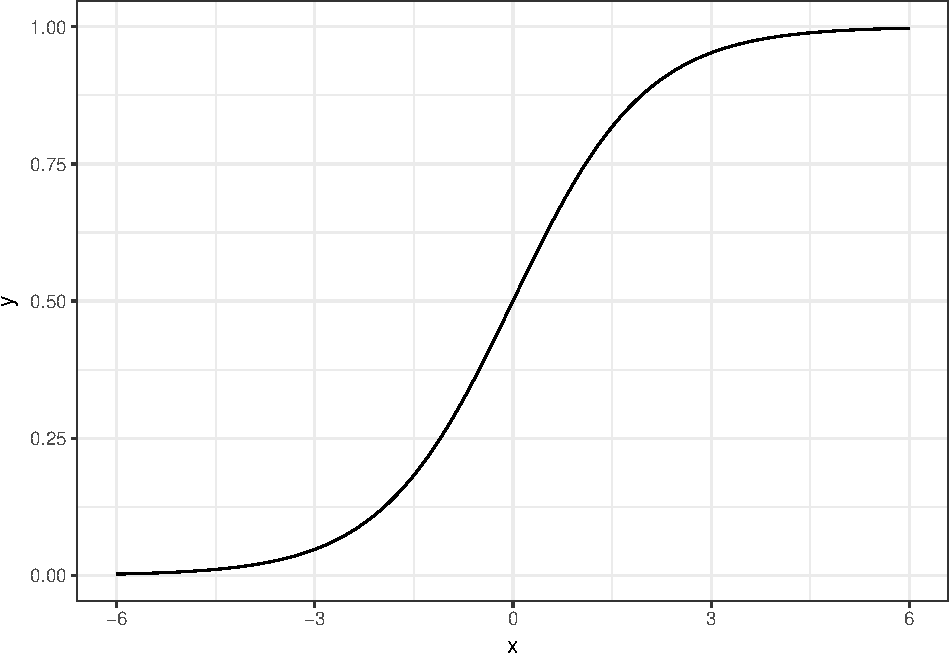
\includegraphics{xai-book_files/figure-latex/logistic-function-1.pdf}
The step from linear regression models to logistic regression is kind of
straightforward. Before we modeled the relationship like this:
\[\hat{y}_{i} = \beta_{0} + \beta_{1} \cdot x_{i,1} + \ldots + \beta_{K} x_{i,K} \]
Now we want probabilities, which are between 0 and 1, so we wrap the
right side of the equation into the logistic regression function and
simply force the output to be between 0 and 1:
\[P(y_{i}=1) =  \frac{1}{1 + exp(-(\beta_{0} + \beta_{1} \cdot x_{i,1} + \ldots + \beta_{K} x_{i,K}))}\]

Let's check the tumor size example again. But now instead of the linear
regression model, we use the logistic regression model:
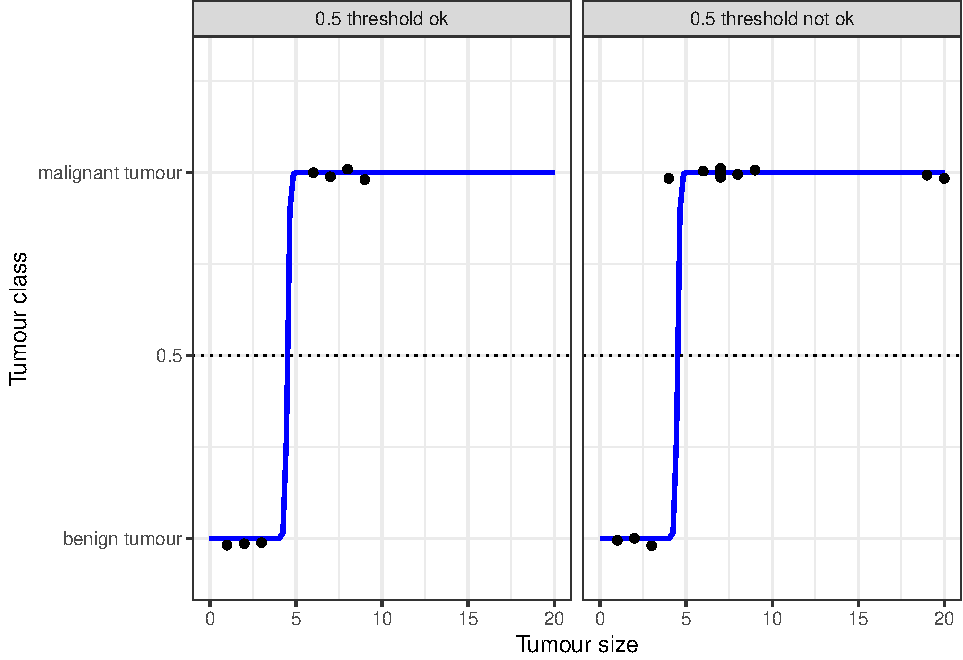
\includegraphics{xai-book_files/figure-latex/logistic-class-threshold-1.pdf}
It works better than with logistic regression and we can use 0.5 as a
threshold. The line does not shift much, when including the additional
datapoints.

\subsection{Interpretation}\label{interpretation-1}

The interpretation of the coefficients differs from linear regression
models. Because now our target value is not some arbitrary number, but a
probability between 0 and 1. Also through the logistic function, the
influence of the features on the target probability has become
non-linear. That's why we need to reformulate the equation for the
interpretation\textgreater{}
\[log\left(\frac{P(y_{i}=1)}{(1 - P(y_{i}=1))}\right) =  log\left(\frac{P(y_{i}=1)}{ P(y_{i}=0)}\right) = \beta_{0} + \beta_{1} \cdot x_{i,1} + \ldots + \beta_{K} x_{i,K}\]
\(\frac{P(y_{i}=1)}{(1 - P(y_{i}=1))}\) is also called odds (probability
of event vs.~probability of no event) and
\(log\left(\frac{P(y_{i}=1)}{(1 - P(y_{i}=1))}\right)\) are the log
odds. So with a logistic regression model we have a linear model for the
log odds. Great! Doesn't sound helpful! Well, with a bit of shuffling
again, you can find out how the prediction changes, when one of the
features \(x{\cdot, k}\) is changed by 1 point. For this we can first
apply the \(exp()\) function on both sides of the equation:
\[\frac{P(y_{i}=1)}{(1 - P(y_{i}=1))} = odds_i =  exp\left(\beta_{0} + \beta_{1} \cdot x_{i,1} + \ldots + \beta_{K} x_{i,K}\right)\]
Then we compare what happens when we increase one of the \(x_{i,j}'s\)
by 1. But instead of looking at the difference, we look at the ratio of
the two predictions, you will see why:
\[ \frac{odds_{i, x_i + 1}}{odds_i}= \frac{exp\left(\beta_{0} + \beta_{1} \cdot x_{i,1} + \ldots + \beta_{k} \cdot (x_{i,k} + 1)  + \ldots+ \beta_{K} x_{i,K}\right)}{exp\left(\beta_{0} + \beta_{1} \cdot x_{i,1} + \ldots + \beta_{k} \cdot x_{i,k}  + \ldots+ \beta_{K} x_{i,K}\right) }  \]
Using the rule that \(\frac{exp(a)}{exp(b)} = exp(a - b)\) gives us:
\[ \frac{odds_{i, x_i + 1}}{odds_i}=exp\left( (\beta_{0} + \beta_{1} \cdot x_{i,1} + \ldots + \beta_{k} \cdot (x_{i,k} + 1)  + \ldots+ \beta_{K} x_{i,K}\right) - \left(\beta_{0} + \beta_{1} \cdot x_{i,1} + \ldots + \beta_{k} \cdot x_{i,k}  + \ldots+ \beta_{K} x_{i,K})\right)\]
And then we can remove a lot of terms from the equation, which is
convenient:
\[ \frac{odds_{i, x_i + 1}}{odds_i}=  exp\left( \beta_{k} \cdot (x_{i,k} + 1) - \beta_{k} \cdot x_{i,k} \right) = exp\left(\beta_k\right)\]

And we end up with something simple like \(\exp(\beta_k)\). So a change
in \(x_k\) by one unit changes the odds ratio (multiplicatively) by a
factor of \(\exp(\beta_k)\). We could also interpret it this way: A
change in \(x_k\) by one unit change the log odds ratio by \(\beta_k\)
units, but most people do the former because thinking in logs is known
to be hard on the brain. Interpreting the odds ratio already needs a bit
of getting used to. If you have odds of 2, it means that the probability
for \(y_i = 1\) is twice as big as \(y_i = 0\). If you have a \(\beta\)
(=odds ratio) of \(0.7\), then an increase in the respective x by one
unit multiplies the odds by \(\exp(0.7) \approx 2\) and your odds would
be 4. But usually you don't deal with the odds and only interpret the
\(\beta\) as the odds ratios. Because for actually calculating the odds
you would need to set a value for each \(x_{i,k}\) for all \(k\), which
only makes sense if you want to look at one specific instance of your
dataset.

Here are the interpretations for the logistic regression model with
different feature types:

\begin{itemize}
\tightlist
\item
  Numerical feature: For an increase of one unit of the feature
  \(x_{j}\) the estimated odds change (multiplicatively) by a factor of
  \(\exp{\beta_{j}}\)
\item
  Binary categorical features: One of the features is the reference
  level (in some languages the one that was coded in 0). A change of the
  feature \(x_{i}\) the reference level to the other category changes
  the estimated odds change (multiplicatively) by a factor of
  \(\exp{\beta_{j}}\)
\item
  Categorical features with many levels: One solution to deal with many
  features is to one-hot-encode them, meaning each level gets it's own
  column. From a categorical feature with L levels, you only need L-1
  columns, otherwise it is over parameterized. The interpretation for
  each level is then according to the binary features. Some language
  like R allow to
\item
  Intercept \(\beta_{0}\): The interpretation is: Given all numerical
  features are zero and the categorical features are on the reference
  level, the estimated odds are is \(\exp{\beta_{0}}\). The
  interpretation of \(\beta_{0}\) is usually not relevant.
\end{itemize}

\subsection{Example}\label{example}

With the logistic regression model we can predict cervical cancer given
risk factors.

\begin{tabular}{l|r|r|r}
\hline
  & Estimate & Odds ratio & Std. Error\\
\hline
Intercept & 2.9101469 & 18.3594963 & 0.3225918\\
\hline
Hormonal contraceptives y/n & 0.1166594 & 1.1237366 & 0.2989597\\
\hline
Smokes y/n & -0.2557759 & 0.7743154 & 0.3719329\\
\hline
Num. of pregnancies & -0.0368039 & 0.9638651 & 0.0965331\\
\hline
Num. of diagnosed STDs & -0.8154926 & 0.4424213 & 0.3260103\\
\hline
Intrauterine device y/n & -0.6163016 & 0.5399376 & 0.3995933\\
\hline
\end{tabular}

Interpretation of a numerical feature (`Num. of diagnosed STDs'): An
increase of the number of diagnosed STDs changes (decreases) the odds
for cancer vs.~no cancer multiplicatively by 0.44, given all other
features stay the same. Keep in mind that correlation does not imply
causation. No recommendation here to get STDs.

Interpretation of a categorical feature (`Hormonal contraceptives y/n'):
For women with hormonal contraceptives, the odds for cancer vs no cancer
are by a factor of 1.12 higher, compared women without hormonal
contraceptives, given all other features stay the same.

Again as in the linear models, the interpretations are always coming
with the clause that `all other features stay the same'.

\section{Decision trees}\label{decision-trees}

Linear models fail in situation where the relationship is non-linear
and/or where the features are interacting with each other. Time to shine
for the decision trees! Tree-based models partition the data along the
features into rectangles. For predicting the outcome in each rectangle
it fits a simple model (for example the average of the outcome of the
instances that fall into this rectangle). Trees have an intuitive
structure starting from a root and splitting into nodes, according to
cutoff values of the features. After each split, the instances fall into
one of the new nodes. At the end of the training all the instances from
the training data set are assigned into one of the leaf nodes. See
Figure @ref\{fig:tree-artificial\} for illustration.

There are a lot of different tree algorithms. They differ in structure
(number of splits per node), criteria for how to find the splits, when
to stop splitting and how to estimate the simple models within the leaf
nodes. Classification and regression trees (CART) is one of the more
popular algorithms for tree building. This book will only talk about
CART, because in the interpretation they are all the same. If you know
of some tree algorithm with a different interpretation, I would welcome
your feedback.

Each of these rectangles is associated with a simple model of the
outcome of the interest. This is usually estimated by taking the mean of
outcomes from all training instances that fall into a rectangle. I
recommend the book `The elements of statistical learning'
\citep{Hastie2009} for a more detailed introduction.

\begin{figure}
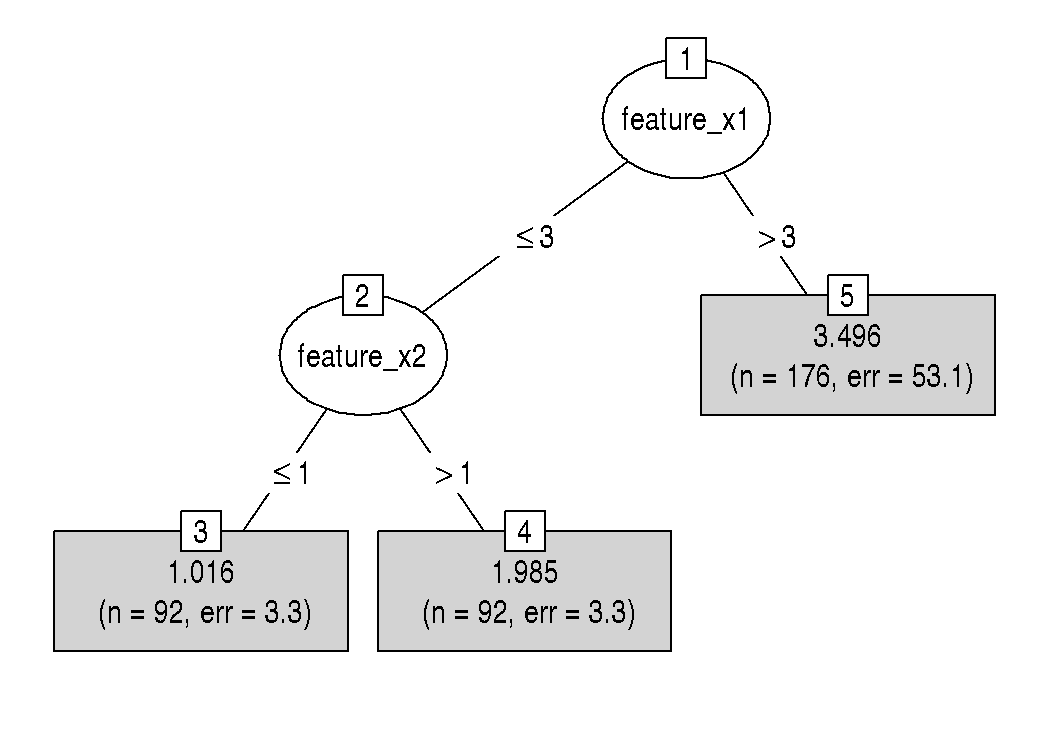
\includegraphics[width=1\linewidth]{xai-book_files/figure-latex/tree-artificial-1} \caption{Exemplary decision tree with artificial data}\label{fig:tree-artificial}
\end{figure}

The following formula describes relationship of y and x (in which
rectangle does x fall?)
\[\hat{y}_i = \hat{f}(x_i) = \sum_{m = 1}^M c_m I\{x_i \in R_m\}\] Each
instance \(x_i\) falls into exactly one leaf node (=rectangle), so
\(I_{\{x_i \in R_m\}}\) is only 1 for the this single leaf node (\(I\)
is the identity function which is 1 if \(x_i \in R_m\) and else 0). If
\(x_i\) falls into leaf node \(R_l\), the predicted outcome
\(\hat{y} = c_l\), where \(c_l\) is the mean of all the training
instances in leaf node \(R_l\).

But where do the `rectangles' come from? This is quite simple: The
algorithm takes a feature and tries which cut-off point minimises the
sum of squares if it is a regression task or the Gini index in
classification tasks. It's the cut-off point that makes the two
resulting subsets as different as possible in terms of the outcome
feature of interest. For categorial features the algorithm tries
different groupings by category into to nodes. After this was done for
each feature, the algorithm looks for the feature with the best cut-off
and chooses this to split the node into two new nodes. The algorithm
continues doing this in both new nodes until the stopping criteria is
reached. Possible criteria are: A minimum number of instances that have
to be in a node before the split, the minimum number of instances that
have to be in a terminal node.

A common strategy is to grow a tree fully and then cut it back to
optimise it's complexity measure \(cp\).

\subsection{Interpretation}\label{interpretation-2}

It's easy: Starting from the root node you go to the next nodes and the
edges tell you which subsets you are looking at. Once you reach the leaf
node, the node tells you the predicted outcome. All the edges are
connected by `AND'.

Template: If feature x is {[}smaller/bigger{]} than threshold c AND
\ldots{}, then the predicted value is \(\hat{y}\).

\subsection{Interpretation example}\label{interpretation-example-1}

Let's have a look again at the speed dating example. Again we want to
predict the rating from the participants, how much they will like the
rating partners.

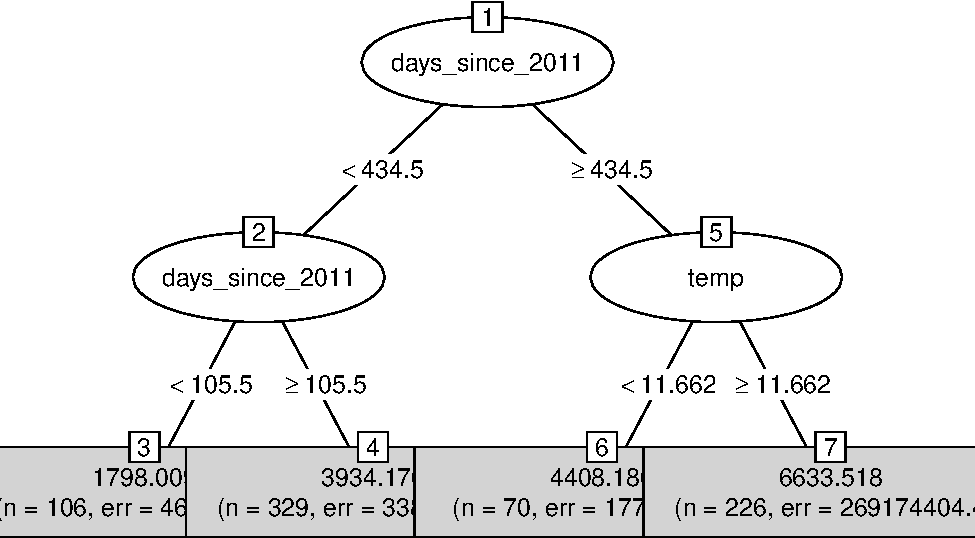
\includegraphics{xai-book_files/figure-latex/tree-example-1.pdf} The
first split was done in the workingday feature, which tells if a day is
a working day or a saturday/sunday/holiday. On days without work, the
number of rental bikes was higher on average. In both child nodes the
the next feature that was chosen was temperature.

In waves of size 20 or smaller, participants who gave 5/10 or more to
importance of same religion of partner, they also rated lower on average
(median around 6). If religion was less important (4 or lower), than
they gave higher ratings.

\subsection{Advantages}\label{advantages}

The tree structure is perfectly suited to \textbf{cover interactions}
between features in the data. The data also ends up in \textbf{distinct
groups}, which are easier to grasp than points on a hyperplane like in
linear regression. The interpretation is arguably pretty
straightforward. The tree structure also has a \textbf{natural
visualization}, with it's nodes and edges.

\subsection{Disadvantages}\label{disadvantages}

\textbf{Handling of real linear relationships}, that's what trees suck
at. Any real linear relationship between an input feature and the
outcome has to be approximated by hard splits, which produces a step
function. This is not efficient. This goes hand in hand with
\textbf{lack of smoothness}. Slight changes in the input feature can
have a big impact on the predicted outcome, which might not be
desirable. Imagine a tree that predicts the worth of a house and the
tree splits in the square meters multiple times. One of the splits is at
100.5 square meters. When a user measure his house and arrives at 99
square meters, types it into some nice web interface and get's 200 000
Euro. The user notices that she forgot to measure a small storeroom with
2 square meters. The storeroom has a skewed wall, so she is not sure if
she can count it fully towards the whole flat area or only half of the
space. So she decides to try both 100.0 and 101.0 square meters. The
results: 200 000 Euro and 205 000 Euro, which is quite unintuitive.

Trees are also quite \textbf{unstable}, so a few changes in the training
data set might create a completely different tree. That's because each
splits depends on the parent split. It does not generate trust if the
structure flips so easily.

\section{Other simple, interpretable
models}\label{other-simple-interpretable-models}

\subsection{Naive bayes classifier}\label{naive-bayes-classifier}

The naive Bayes classifier make use of the Bayes'theorem. For each
feature it computes the probability for a class given the features
value. The clue is that naive Bayes does so for each feature
independently, which is the same as having a strong (=naive) assumption
of independence of the features. Naive Bayes is a conditional
probability model and models the probability of a class \(k\) in the
following way:
\[ P(C_k|x) = \frac{1}{Z} P(C_k) \prod_{i=1}^n P(x_i | C_k)\]

The term \(Z\) is a scaling parameter that ensures that the
probabilities for all classes sum up to 1.

Naive Bayes is an interpretable model, because of the independence
assumption. For each classification it is very clear for each feature
how much it contributes towards a certain class prediction.

\subsection{k-nearest neighbours}\label{k-nearest-neighbours}

k-nearest neighbour can be used for regression and classification and
uses the closest neighbours for a data point for prediction. For
classification it assigns the class most common the closest \(k\)
neighbours of an instance and for regression it takes the average of the
outcome. The tricky parts are finding the right \(k\) and defining the
neighbourhood. This algorithm is different from the other intepretable
models presented in this book, since it is an instance-based learning
algorithm. How is k-nearest neighbour interpretable? For starters, there
is no global model interpretability, since the model is inherently local
and there are no global weights or structures that are learned
explicitly by the k-nearest neighbour method. Maybe it is interpretable
on a local level? To explain a prediction, you can always retrieve the
k-neighbours that were used. If this is interpretable solely depends if
you can `interpret' single instances in the dataset. If the dataset
consists of hundreds or thousands of features, then it is not
interpretable I'd argue. But if you have few features or a way to reduce
your instance to the most important features, presenting the k-nearest
neighbours can give you good explanations.

\subsection{RuleFit}\label{rulefit}

The RuleFit algorithm from Friedman and Propescu
\citep{friedman2008predictive} is a regression and classification
approach that uses decision rules in a linear model. RuleFit consists of
two components: The first component produces ``rules'' and the second
component fits a linear model with these rules as input (hence the name
``RuleFit''). It enables automatic integration of interactions between
features into a linear model, while having the interpretability of a
sparse linear model.

There are two steps involved:

Step 1: Rule generation:

The rules that the algorithm generates have a simple form:

if \(x2 < 3\) and \(x5 < 7\) then \(1\) else \(0\)

The rules are generated from the covariates matrix X. You can also see
the rules simply as new features based on your original features.

The RuleFit paper uses the Boston housing data as example: The goal is
to predict the median house value in the Boston neighborhood. One of the
rules that is generated by RuleFit is:

if (number of rooms \(> 6.64\)) and (concentration of nitric oxide
\(< 0.67\)) then \(1\) else \(0\)

The interesting part is how those rules are generated: They are derived
from Decision Trees, by basically disassembling them. Every path in a
tree can be turned into a decision rule. You simply chain the binary
decisions that lead to a certain node, et voilà, you have a rule. It is
desirable to generate a lot of diverse and meaningful rules. Gradient
boosting is used to fit an ensemble of decision trees (by
regressing/classifying y with your original features X). Each resulting
trees is turned into multiple rules.

\begin{figure}
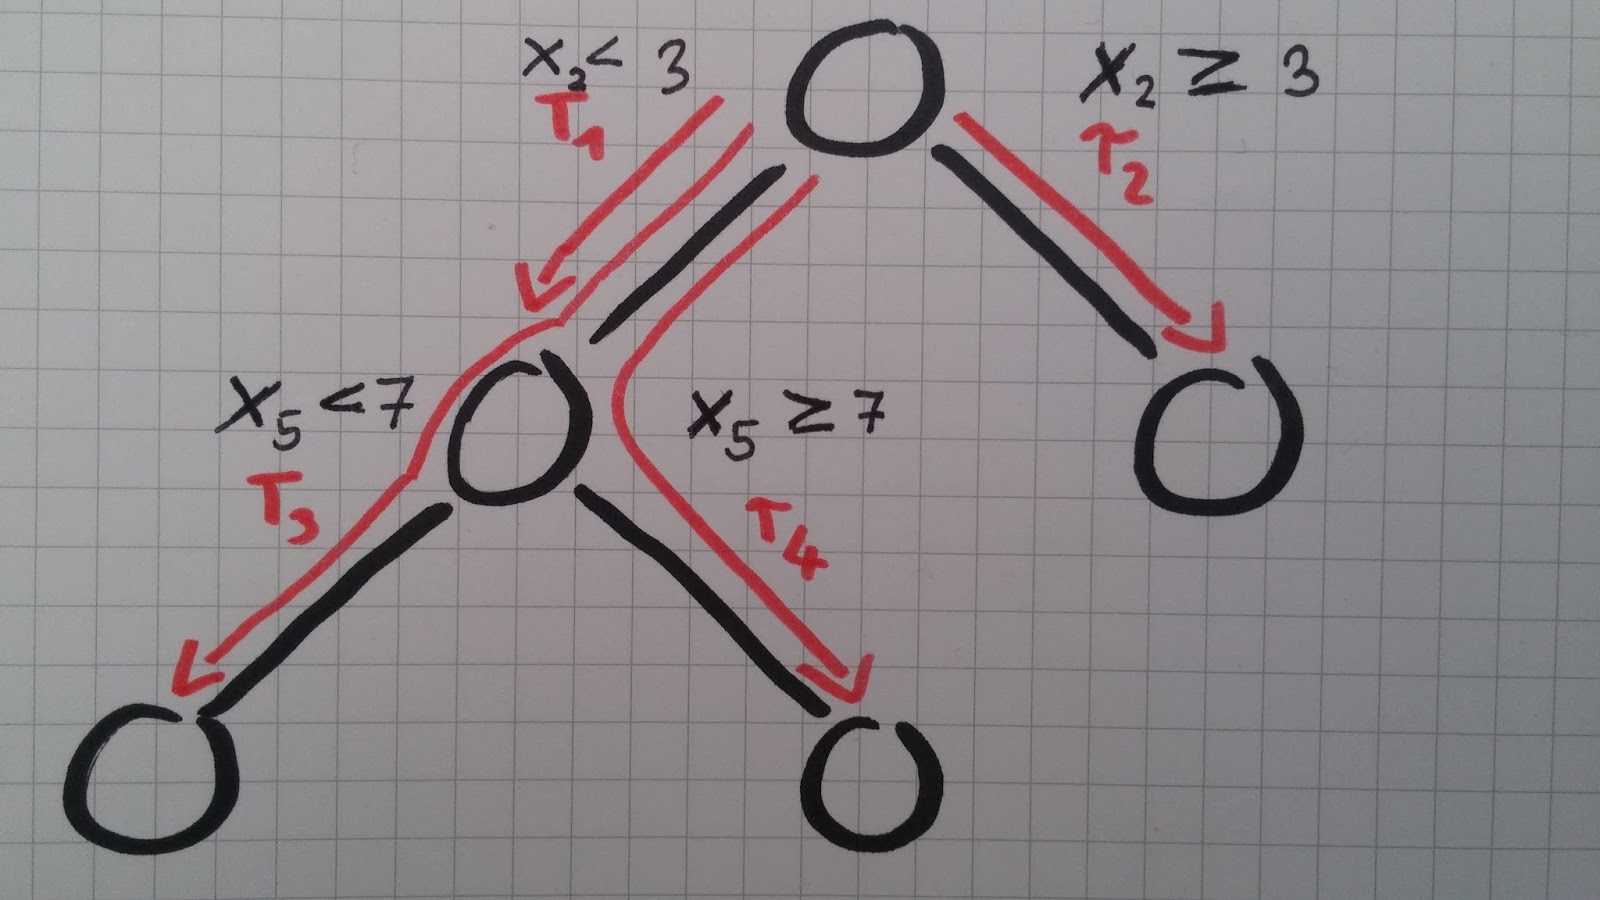
\includegraphics[width=0.8\linewidth]{images/rulefit} \caption{4 rules can be generated from a tree with 3 terminal nodes.}\label{fig:rulefit}
\end{figure}

Another way to see this step is a black box, that generates a new set of
features X' out of your original features X. Those features are binary
and can represent quite complex interactions of your original X. The
rules are chosen to maximise the prediction/classification task at hand.

Step 2: Sparse linear model

You will get A LOT of rules from the first step (and that is what you
want). Since the first step is only a feature transformation function on
your original data set you are still not done with fitting a model and
also you want to reduce the number of rules. Lasso or L1 regularised
regression is good in this scenario. Next to the rules also all
numerical features from your original data set will be used in the Lasso
linear model. Every rule and numerical feature gets a coefficient
(beta). And thanks to the regularisation, a lot of those betas will be
estimated to zero. The numerical features are added because trees suck
at representing simple linear relationships between y and x. The outcome
is a linear model that has linear effects for all of the numerical
features and also linear terms for the rules.

The interpretation is the same as with linear models, the only
difference is that some features are now binary rules.

The paper not only introduces RuleFit and evaluates it, but it also
comes with a bunch of useful tools, (comparable to Random Forest):
Measurement tools for feature importance, degree of relevance of
original input features and interaction effects between features.

\subsection{And so many more \ldots{}}\label{and-so-many-more}

There are lots and lots of algorithms that produce interpretable models
and not all will be listed here. If you are a researcher or just a big
fan and user of a certain interpreable method that is not listed here,
get in touch with me and add the method to this book!

\chapter{Model-agnostic tools for interpretability}\label{agnostic}

Separating the explanations from the machine learning model (=
model-agnostic explanations) gives some benefits. The big advantage of
model-agnostic vs model-specific explanation algorithm is the
flexibility. When the explanation system is independently applicable
even when the underlying model is switched, it frees the practitioner to
use different machine learning models without restrictions. It is also
more efficient to build interfaces on top of model-agnostic systems,
because this has to be done only once and not for each model-specific
explanation system. Usually not one but many types of machine learning
models are tested in development time and if you want to compare the
models in terms of interpretability this is easier with model-agnostic
explanations because the system is the same for both models that are
being compared \citep{Ribeiro2016b}.

The alternatives are either using only interpretable models as
introduced in Chapter 2, which has the big disadvantage to usually loose
accuracy compared to other approaches. The other alternative is to use
more flexible model classes that come with built in explanations. The
drawback here is that it ties you to this one algorithm and it will be
hard to switch to something else.

Desirable aspects of a model-agnostic explanation system
\citep{Ribeiro2016b}: - Model flexibility: Not being tied to an
underlying particular machine learning model. The method should work for
random forests as well as convolutional neural networks - Explanation
flexibility: Not being tied to a certain form of explanation. In some
cases it might be useful to have a linear formula in other cases some
decision rules - Representation flexibility: The explanation system
should not have to use the same feature representation as the model that
is being explained. So when a text classifier uses abstract word
embedding vectors, it might be preferable to use the presence of single
words for the explanation.

\textbf{The bigger picture}

Let's take a high level view on model-agnostic interpretability. Figure
\ref{fig:bigpicture} shows how we first abstract the world by capturing
it by collecting data and abstract it further by learning the essence of
the data (for the task) with a machine learning model. Interpretability
is just another layer on top, that helps humans understand.

\begin{itemize}
\tightlist
\item
  The bottom layer is the `World'. This could literally be nature
  itself, like the biology of the human body and how it reacts to
  medication, but also more abstract things like the real estate market.
  The `World'-layer contains everything that can be observed and is of
  interest. Ultimately we want to learn something about the `World' and
  interact with it.
\item
  The second layer is the `Data'-layer. We have to digitalise the
  `World' in order to make it processable for computers and also to
  store information. The `Data'-layer contains anything from images,
  texts, tabular data and so on.
\item
  By fitting machine learning models on top of the `Data'-layer we get
  the `Black Box Model'-layer. Machine learning algorithms learns with
  data from the real world to make predictions or find structures.
\item
  On top of the `Black-Box-Layer' is the `Interpretable Methods' layer
  that helps us deal with the opaqueness of machine learning models.
  What were the important attributes for a particular diagnosis? Why was
  a financial transaction classified as fraud?
\item
  The last layer is occupied by a `Human'. Look! This one is waving at
  you because you are reading this book and you are helping to provide
  better explanations for black box models! Humans are the consumers of
  the explanations ultimately.
\end{itemize}

\begin{figure}
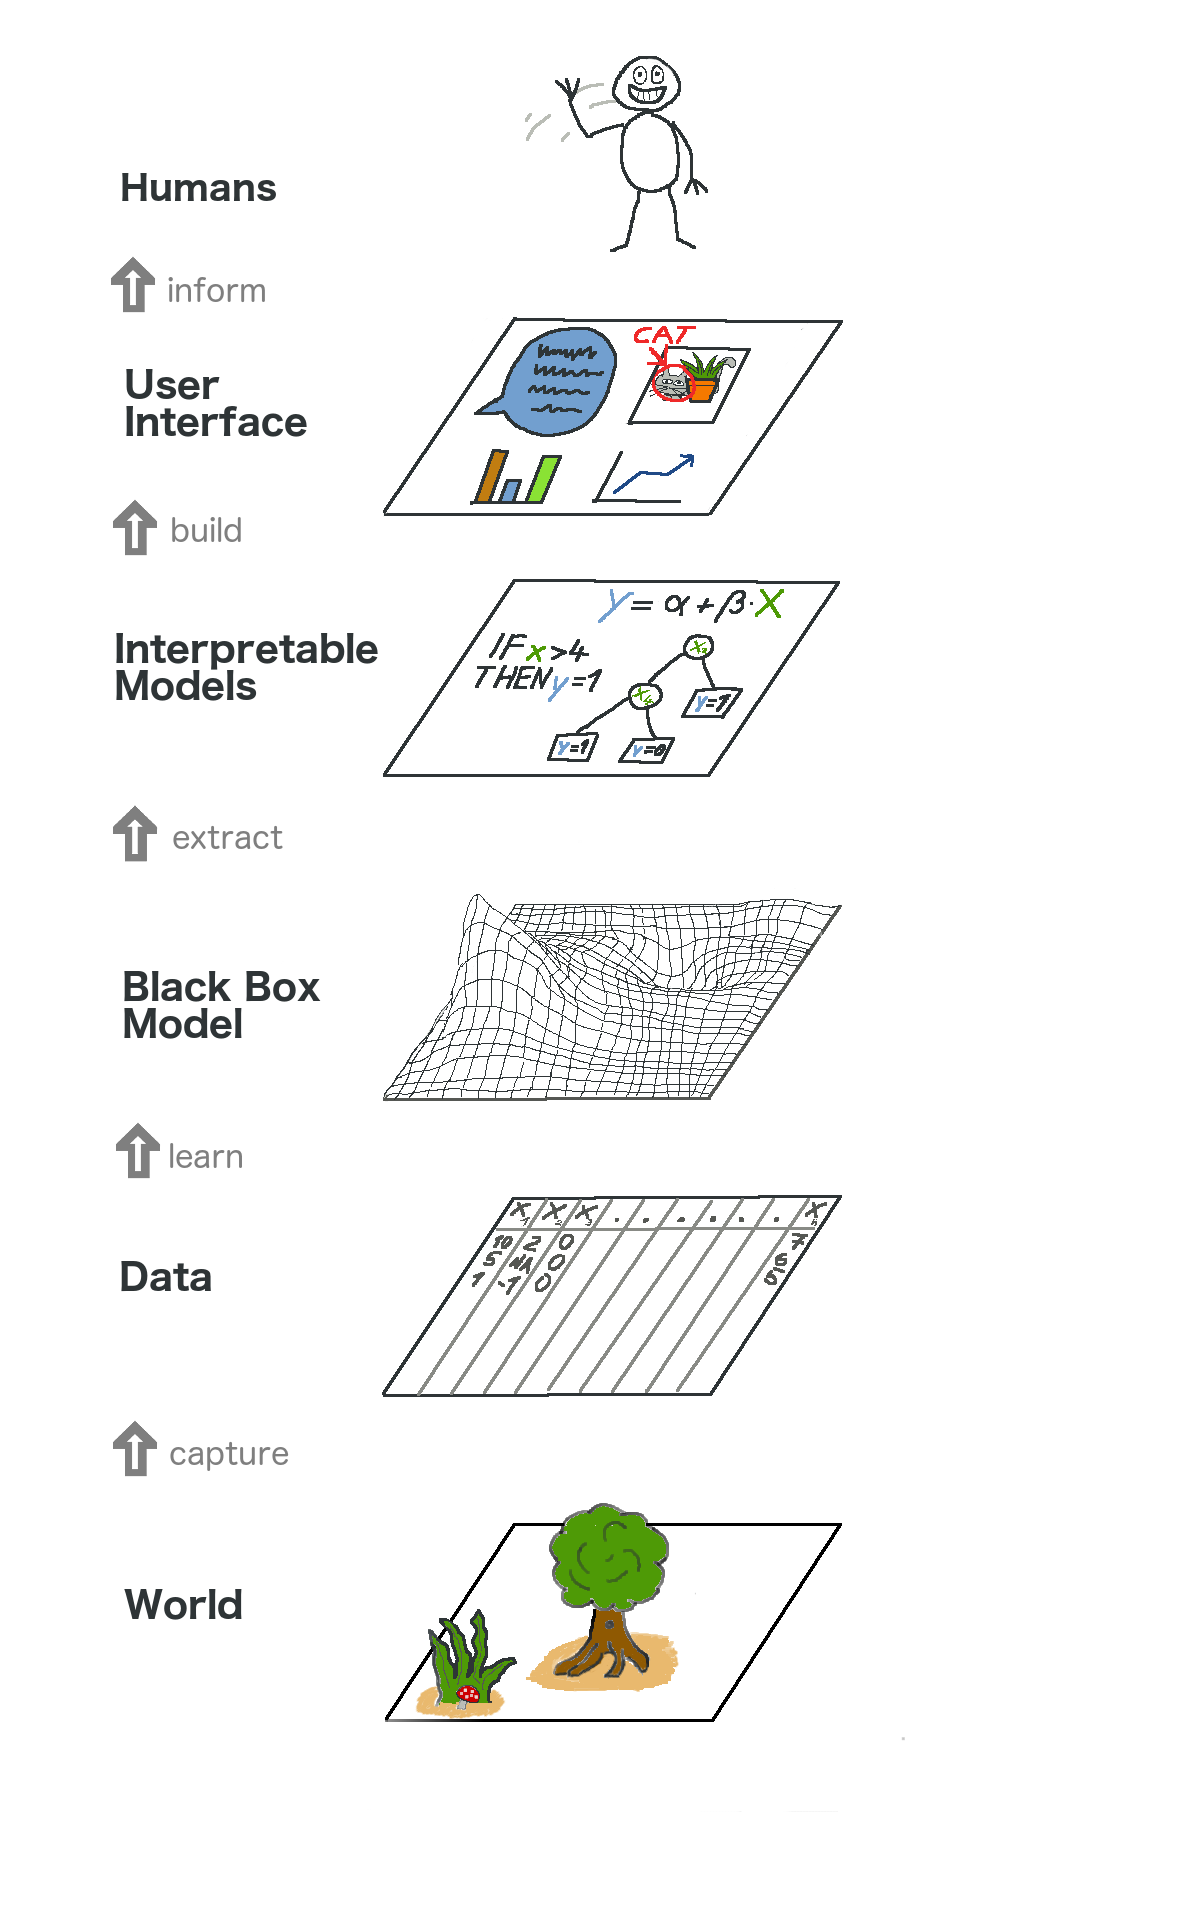
\includegraphics[width=0.8\linewidth]{images/big-picture} \caption{The big picture of explainable machine learning. The real world goes through many layers before it reaches the human in forms of explanations.}\label{fig:bigpicture}
\end{figure}

This layered abstraction also helps in understanding what the
differences in approaches between statisticians and machine learning
practitioners is. Statistician are concerned with the `Data' layer, like
planning clinical trials or designing surveys. The they skip the `Black
Box Model'-layer and go right to the `Interpretable Methods' and from
there to the explanations for our human. Machine learning specialists
are also concerned with the `Data'-layer, like collecting labeled
samples of skin cancer images or crawling Wikipedia. Then comes the
machine learning model. `Interpretable models' and `Explanations' are
skipped and the human deals directly with the `Black Box Model'. It's a
nice thing, that in explainable machine learning, the work of a
statistician and a machine learner fuses and becomes something better.

Of course this graphic does not capture everything: Data could come from
simulations. Black box models also output predictions that might not
even reach humans, but only feed other machines and so on. But overall
it is a useful abstraction for understanding how (model-agnostic)
interpretability becomes this new layer on top of machine learning
models.

\section{Partial dependence plot}\label{pdp}

The partial dependence plot shows the marginal effect of a variable on
the target (regression / classification) \citep{friedman2001greedy}. A
partial dependence plot can show if the relationship between target and
feature is linear, monotonic or something else. In linear regression,
those plots will always show a linear relationship.

The partial dependence function for regression is defined as:
\[f_S = E_{x_C}[f(x_S, x_C)] = \int f(x_S, x_C) dP(x_C)\] The \(x_S\) is
the set of variables for which the partial dependence should be depicted
and \(x_C\) are the other variables that were used in the machine
learning model. Partial dependence works by averaging out the other
variables, so that the remaining function shows the relationship between
the \(x_S\), in which we are interested, and the target. \(x_S\) is
fixed and \(x_C\) is varying.

The integral is estimated by calculating averages in the training data,
which looks like this for regression:
\[ \hat{f}(x_S) = \frac{1}{n} \sum_{i=1}^n f(x_S, x_{Ci}) \] In this
formula, \(x\) is the variable for which to calculate the partial
dependence, \(x_{iC}\) is the other variables and \(n\) the number of
instances in the data set.

For classification it is the logits:
\[ f(x) = \log p_k(x) - \frac{1}{K} \sum_{j=1}^K \log p_j(x) \]

Partial dependence plots are only partially global: They are global
because they take into account all instances, but it is local in the
feature, because partial dependence plots only examine one variable, as
the name suggests.

\subsubsection{Examples}\label{examples}

In practice \(x_S\) usually only contains one variable or a maximum of
two, because one variable produces 2D plots and two variables produce 3D
plots. Everything beyond that is quite tricky. Even 3D on a 2D paper or
monitor is already challenging. This example here shows an artificial
dataset with two x variables on which a Random Forest was trained.

\begin{figure}
\centering
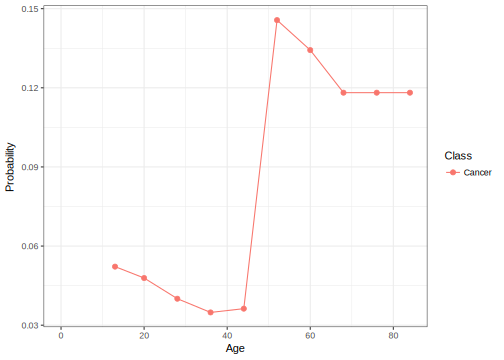
\includegraphics{xai-book_files/figure-latex/dpd-cervical-1.pdf}
\caption{\label{fig:dpd-cervical}Partial dependence plot of cancer
probability and different factors. For the age feature, the models
partial dependence shows that on average, the cancer probability is low
before 45, spikes between age 45 and 55 and plateaus after that.}
\end{figure}

\begin{figure}
\centering
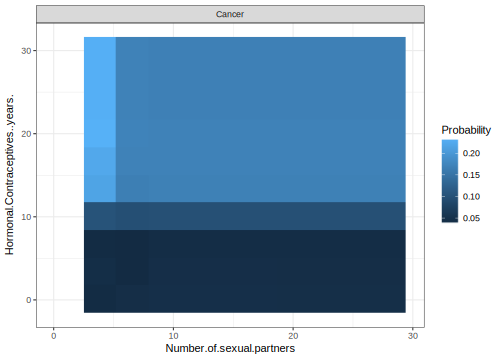
\includegraphics{xai-book_files/figure-latex/dpd-cervical-2d-1.pdf}
\caption{\label{fig:dpd-cervical-2d}Partial dependence plot of cancer
probability and the interaction of number of years on hormonal
contraceptives and number of sexual partners. Interestingly, there is
some odd interaction between the two variables when the number of sexual
partners is 1 and the years of on hormonal contraceptives larger than
12. There are actually only two women in that group, who both happen to
have cancer. So my best guess is that this was random and the model did
overfit on those two women, but only more data could solve this
question.}
\end{figure}

Let's turn to the regression example with the bike counts again and have
a look at how the weather effects look like. @ref\{fig:dpd-bike\} shows
the average influence of the weather features on the predicted bike
counts. Warm, but not too hot weather makes the model predict a high
number of bikes rentals. The potential bikers are increasingly inhibited
in engaging in cycling when humidity reaches above 60\%. Also the more
wind the less people like to bike, which personally I can understand.
Interestingly the predicted bike counts don't drop between 25 and 35
km/h, but maybe there is just not enough training data. At least
intuitively I would expect the bike rentals to drop with each increase
in windspeed, especially when the windspeed is very high.

\begin{figure}
\centering
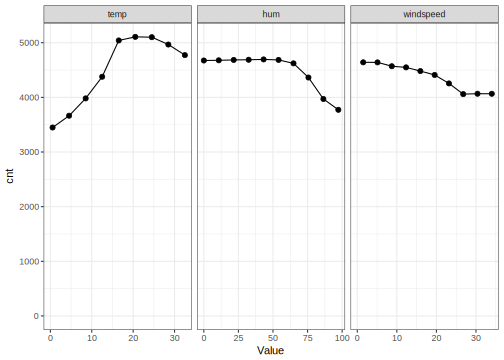
\includegraphics{xai-book_files/figure-latex/dpd-bike-1.pdf}
\caption{\label{fig:dpd-bike}Partial dependence plot of rental bike count
and different weather measurements (Temperature, Humidity, Windspeed).
The biggest differences can be seen in different temperatures: With
rising temperatures, on average the bike rentals rise, until 20C
degrees, where it stays the same also for hotter temperatures and drops
a bit again towards 30C degrees.}
\end{figure}

\section{Individual Conditional Expectation (ICE)
plot}\label{individual-conditional-expectation-ice-plot}

The partial dependence plot is for visualizing the averaged effect of a
feature is a global method, because it does not focus on the partial
dependence of a specific instance, but on an average over all. The
equivalent to a PDP for local expectations is called individiual
conditional expectation (ICE) plot \citep{goldstein2015peeking}. An ICE
plot visualizes the dependence of each instance's predicted response on
a feature. They are event simpler than PDPs, since no averaging is
needed. Instead of drawing one line for a feature, each instance in the
dataset gets it's own line. The values for a line can be computed
easily, by leaving all other features the same, but creating variants of
the instance of interest and letting the black box make the predictions
or classifications. The result is a set of points for a varying feature,
for one specific instance. The lines for the instances can look quite
differently (if the black box allows interactions between features),
because the course of the line depends on the specific values of each
instance. For drawing each line, the \(x_C\) are fixed for this one
instance, and the \(x_C\) is varied on a grid and the \(\hat(y)\)
calculated with \(\hat(f)\).

So, what do you gain by looking at individual expectations, instead of
partial dependencies? This averaged display can obfuscate a
heterogeneous relationship that comes from interactions. ICE plots
\citet{goldstein2015peeking} solve this problem by plotting the
relationship between feature and predicted response for individual
instances. It can be seen as an extension to the standard PDP. PDP can
show you how the average relationship between feature \(x_S\) and
\(\hat(y)\) looks like. This works only well in cases where the
interactions between \(x_S\) and the remaining \(x_C\) are weak. If
there are interactions, a ICE plot will give a lot more insight.

A more formal definition: In ICE plots, for each instance in
\(\{(x_{S_i}, x_{C_i})\}_{i=1}^N\) the curve \(\hat{f}_S^{(i)}\) is
plotted against \(x_{S_i}\), while \(x_{C_i}\) is kept fixed. \#\#\#\#
Example Let's go back to the dataset about risk factors for cervical
cancers and see how each instance's prediction is associated with the
feature `Age'. In the partial dependence plot chapter \ref{pdp} we have
seen that the probability increases around the age of 50, but does this
hold true for each woman in the dataset? The ICE plot reveals that the
most women's predicted probability follows the average pattern of
increase at 50, but there are a few exceptions: In a few cases, the
prediction of cancer probability does not change much with the age, and
that is for women that have a high predicted probability.
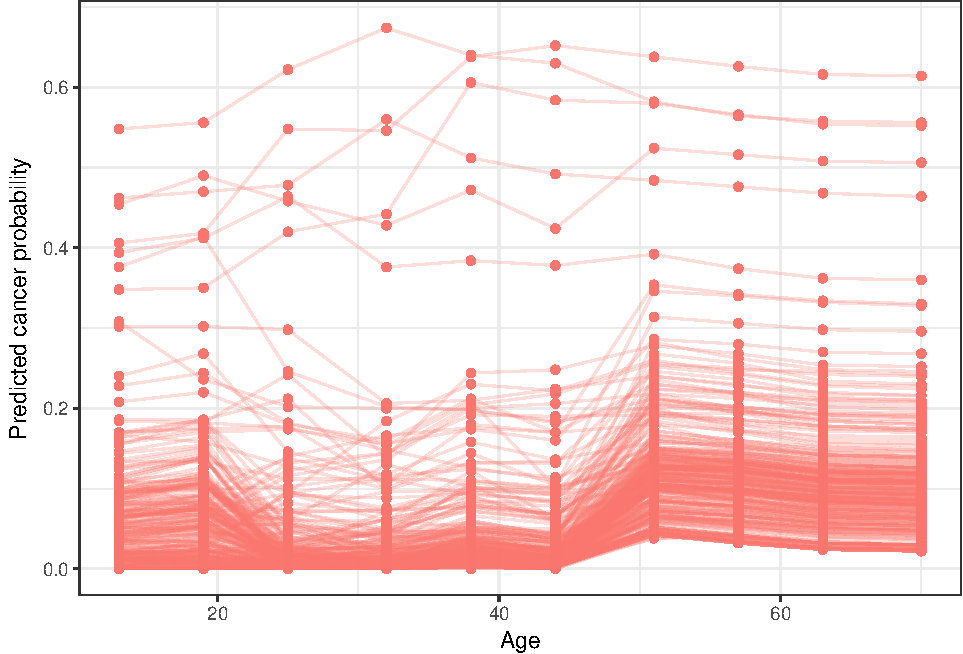
\includegraphics{xai-book_files/figure-latex/ice-cervical-1.pdf}

\begin{figure}
\centering
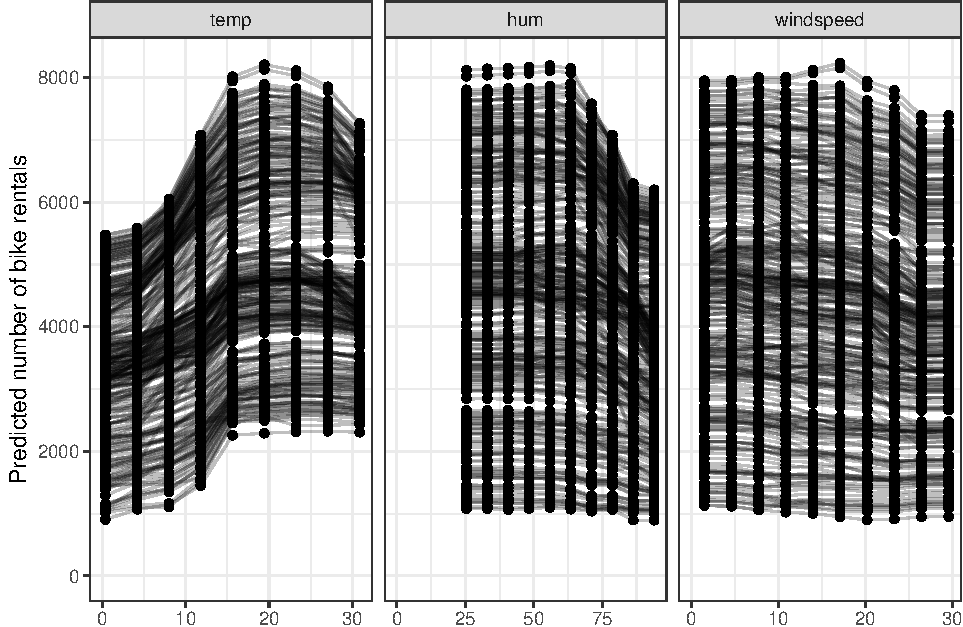
\includegraphics{xai-book_files/figure-latex/ice-bike-1.pdf}
\caption{\label{fig:ice-bike}Individual conditional expectation plot of
expected bike rentals and weather conditions . Same effects as in the
partial dependence plot can be seen.}
\end{figure}

\subsubsection{Centered ICE plot}\label{centered-ice-plot}

There is one issue with the ICE plot: It can be hard to see if the
individual conditionl expectations curve differ between individuals when
they start at different \(\hat{f^{(i)}}\). An easy fix is to center the
curves at a certain point in \(x_S\) and only display the difference in
predited response. The resulting plot is called centered ICE plot
(c-ICE). It is a kind of anchoring, and doing this at the lower end of
\(x_S\) is a good choice. The new curves are defined as:
\[\hat{f}_{cent}^{(i)} = \hat{f}_i - 1\hat{f}(x^{\text{*}}, x_{C_i}), \]
where \(1\) is a vector of 1's with the appropriate dimensions (usually
one- or two-dimensional), and \(\hat{f}\) the fitted model.

\subsubsection{Example}\label{example-1}

Taking Figure @ref\{fig:ice-cervical\} and centering the lines at the
youngest observed age yields Figure @ref\{fig:ice-cervical-centered\}.
It is easier to see now, how the relative change of the curves from the
youngest age is. This can be useful when we are not interested in seing
the absolute change of a predicted value, but rather the difference in
prediction compared to a fixed point of the feature range.
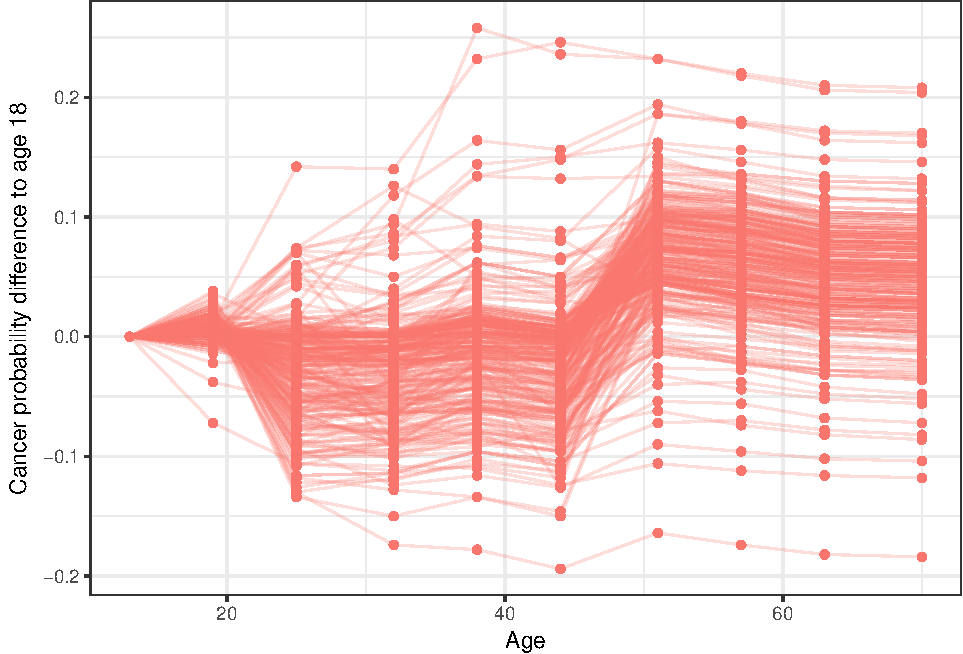
\includegraphics{xai-book_files/figure-latex/ice-cervical-centered-1.pdf}

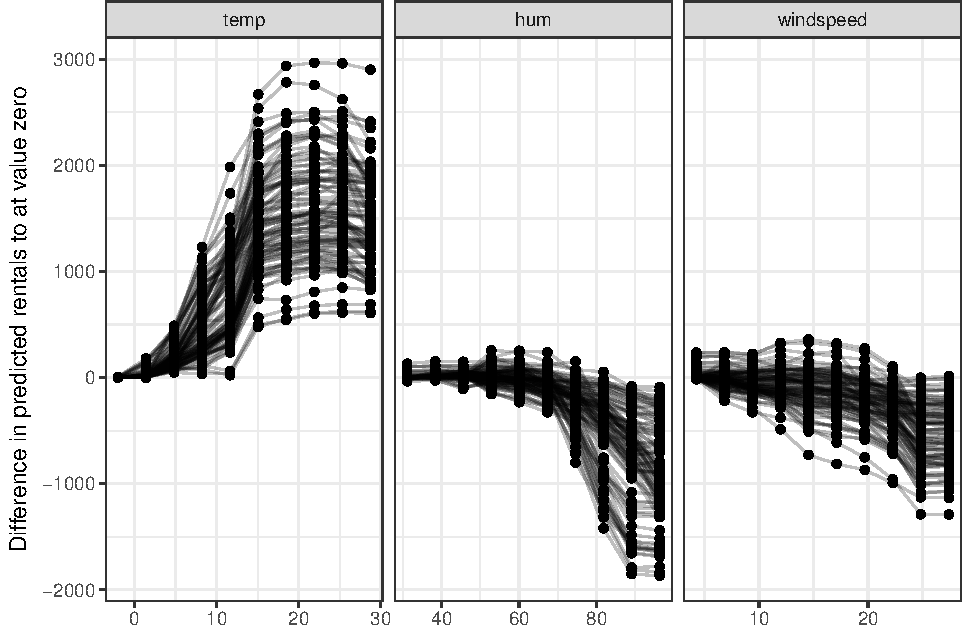
\includegraphics{xai-book_files/figure-latex/ice-bike-centered-1.pdf}
\#\#\#\# Derivative ICE plot Another way to make it it visually easier
to spot heterogenity is to look at the individual derivatives of
\(\hat(f)\) with respect to \(x_S\) instead of the predicted response
\(\hat(f)\). The resulting plot is called derivative ICE plot (d-ICE).
The derivatives of a function (or curve) tells you in which direction
changes occur and if any occur at all. With the derivative ICE plot it
is easy to spot value ranges in a feature where the black box's
predicted value changes for (at least some) instances. If there is no
interaction between \(x_S\) and \(x_C\), then \(\hat{f}\) can be
expressed as:
\[\hat{f}(x) = \hat(f)(x_S, x_C) = g(x_S) + h(x_C), \text{ so that } \frac{\delta\hat{f}(x)}{\delta x_S} = g'(x_S)\]
Without interactions, the individual partial derivatives should be the
same for all instances. If they differ, it's because of interactions and
it will become visible in the d-ICE plot. In addition to displaying the
individual curves for derivative \(\hat{f}\), showing the standard
deviation of derivative \(\hat{f}\) helps to highlight regions in
\(x_S\) with heterogeneity in the estimated derivatives.

\citep{goldstein2015peeking}

\subsubsection{Example}\label{example-2}

As we have seen, the most changes in estimated cancer probability happen
around age 45. This is confirmed by the derivative ICE plot in Figure
@ref\{fig:ice-cervical-derivative\}.
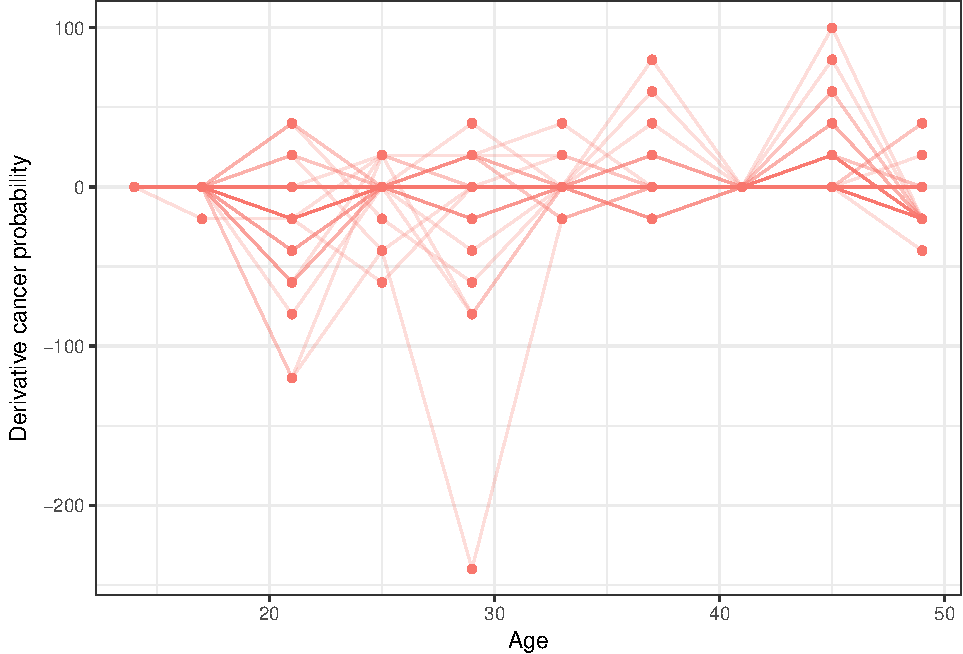
\includegraphics{xai-book_files/figure-latex/ice-cervical-derivative-1.pdf}

\begin{figure}
\centering
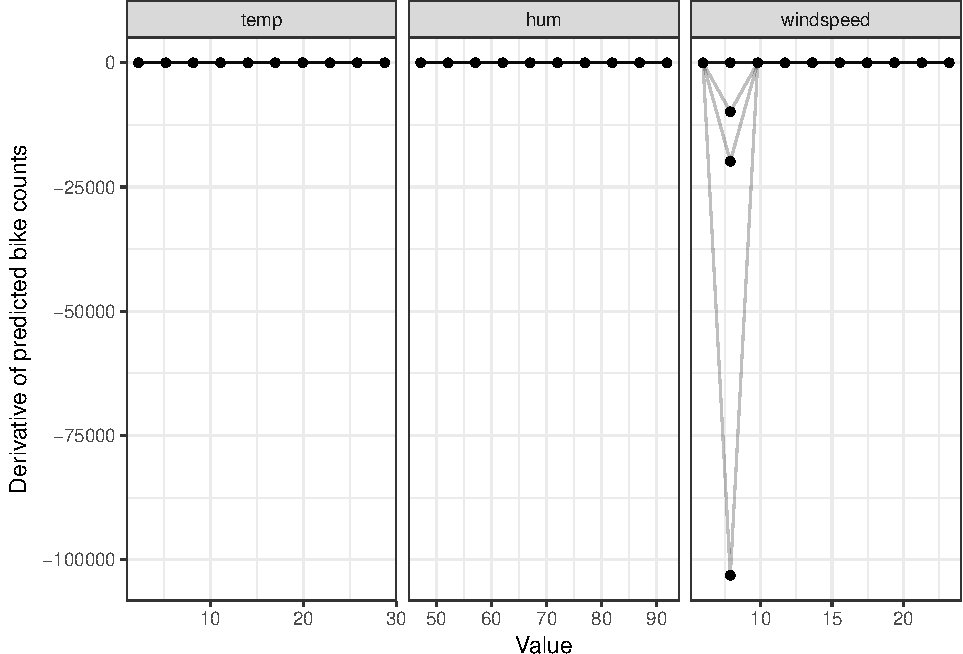
\includegraphics{xai-book_files/figure-latex/ice-bike-derivative-1.pdf}
\caption{\label{fig:ice-bike-derivative}Derivative individual conditional
expectation plot of expected bike rentals and weather conditions.}
\end{figure}

\section{Permutation feature
importance}\label{permutation-feature-importance}

The permutation importance measurement was orginially introduced for
RandomForests \citep{breiman2001random}. It is calculated on the
out-of-bag instances and works by estimating the original model
performance and checking what happens with the model performance when
you permute each feature. A big loss in performance means a big feature
importance. The idea of permutation of features is per se
model-agnostic, only the OOB-scheme is specific for ensemble methods. In
can be used for any model when a hold-out dataset is used, instead of
OOB samples. Of course you could also use the training data, but you
risk getting variable importance measures that overfit your training
data, since the model was already trained on it.

Algorithm \citep{breiman2001random}:

Input: Trained model \(\hat{f}\), hold-out dataset \(D\), number of
permutations \(n_{perm}\)

\begin{enumerate}
\def\labelenumi{\arabic{enumi}.}
\tightlist
\item
  Estimate performance \(Perf\) of \(\hat{f}\) with \(D\) (e.g.~MSE for
  regression or accuracy for classification)
\item
  For each feature \(j \in 1, \ldots, J\) do:
\end{enumerate}

\begin{itemize}
\tightlist
\item
  For \(i \in 1,\ldots , n_{perm}\)

  \begin{itemize}
  \tightlist
  \item
    Get \(D_{j_{perm}}\) by permuting feature \(X_j\) in data \(D\).
    This breaks the association between \(X_j\) and \(Y\).
  \item
    Estimate performance \(Perf_{i,j_{perm}}\) of \(\hat{f}\) with
    \(D_{j_{perm}}\)
  \item
    Calculate permutation variable importance
    \(VI_i(X_j) = Perf_{i,j_{perm}} - Perf\)
  \end{itemize}
\item
  Calculate mean variable importance:
  \(VI(X_j) = \frac{1}{n_{perm}}\sum_{i=1}^{n_{perm}} VI_i(X_j)\)
\item
  Optional: Calculate p-value
  \(p = \frac{I(Perf_{j_{perm}} > Perf)}{n_{perm}}\)
\end{itemize}

\begin{enumerate}
\def\labelenumi{\arabic{enumi}.}
\setcounter{enumi}{2}
\tightlist
\item
  Sort variables by descending \(VI\).
\end{enumerate}

The feature with the highest \(VI\) measure is the most important
globally in your model. With the p-value you can additionally check if a
feature importance is significantly different from 0. You might want to
adjust your \(\alpha\) confidence level for multiple testing.

You can also find the algorithm in more detail in \citep{Strobl2008}.
The authors additionally suggest a conditional feature importance
measurement, which is not (yet) covered in this book. The standard
permutation feature importance only works with marginal feature
improvements and cannot distinguish between correlation and spurious
correlation. \citep{Strobl2008} suggest to condition the importance
measure also on other features, which makes it possible to account for
correlation among the features.

\subsection{Model dependent feature
importance}\label{model-dependent-feature-importance}

Some model classes already come with built in feature importance
measurements. A few examples: - RandomForest: Permutation based feature
importance - CART and boosting: mean decrease in Gini impurity index -
Linear Model: (absolute value of) t-test statistic for each feature

\section{Local surrogate models
(LIME)}\label{local-surrogate-models-lime}

Local interpretable model-agnostic explanations (LIME) is a method for
fitting local, interpretable models that can explain single predictions
or classifications of any black-box machine learning model. LIME
explanations are local surrogate models. Instead of trying to fit a
global surrogate model, LIME focuses on a prediction done by a black-box
algorithm and explains it's outcome.

The idea is quite simple, really. First of all, forget about the
training data and imagine you only have the black box model where you
can input data points and get the models outcome. You can probe the box
as often as you want. Your goal is to understand why the machine
learning model gave the outcome it produced. LIME tests out what happens
to the model's predictions when you put some variations of your data
point of interest into the machine learning model. This basically
generates a new dataset consisting of the perturbed samples and the
associated model's outcome. On this dataset LIME then trains a simple
model weighted by the proximity of the sampled instances to the instance
of interest. The simple mode can basically be any from Section
{[}\#simple{]}, for example LASSO or a short tree. The learned model
should be a good approximation of the machine learning model locally,
but it does not have to be so globally. This kind of accuracy is also
called local fidelity.

The recipe:

\begin{itemize}
\tightlist
\item
  Choose your instance of interest for which you want to have an
  explanation of it's black box outcome
\item
  Make some variations of the instances and check what the black box
  predicts in the neighbourhood of the instance of interest.
\item
  Fit a local, interpretable model on the dataset with the variations
\item
  Explain prediction by interpreting the local simple model.
\end{itemize}

In the current implementation, only LASSO can be chosen as a simple
model. Upfront you have to choose K, the number of features that you
want to have in your simple model. The lower the K, the simpler the
model is to understand, higher K potentially creates models with higher
fidelity. There are different methods for how to fit models with exactly
K features. The most natural with LASSO is the lasso path. Starting from
a model with a very high regularisation parameter \(\lambda\) yields a
model with only the intercept. By refitting the LASSO models with slowly
decreasing \(\lambda\) one after each other the features are getting
weight estimates different from zero. When K features are in the model,
you reached the desired number of features. Other strategies are forward
or backward selection of features. This means you either start with the
full model (=containing all features) or with a model with only the
intercept and then testing which feature would create the biggest
improvement when added or removed, until a model with K features are
reached. Other simple models like decision trees are currently not
implemented.

As always, the devil is in the details. In a high-dimensional space,
defining a neighbourhood is not trivial. Distance measures are quite
arbitrary and distances in different dimensions (aka features) might not
be comparable at all. How big should the neighbourhood be you look into?
If it is too small, then there might be no difference in the predictions
of the machine learning model at all. The other question is: How do you
get the variations of the data? This differs depending on the type of
data, which can be either text, an image or tabular data. For text and
image the solution is turning off and on single words or superpixels. In
the case of tabular data LIME creates new samples by pertubing each
feature individually, by drawing from a normal distribution with mean
and standard deviation from the feature.

\subsubsection{LIME for tabular data}\label{lime-for-tabular-data}

Tabular data means any data that comes in tables, where each row
represents an instance and each column a feature. Sampling is not done
around the point, but from the training data's mass center. Has it's
problems. But it increases the likelihood that the outcome for some of
the sampled points predictions differ from the data point of interest
and that LIME can learn at least some explanation.

Figure \ref{fig:lime-fitting} explains how the sampling and local model
fitting works.

\begin{figure}
\centering
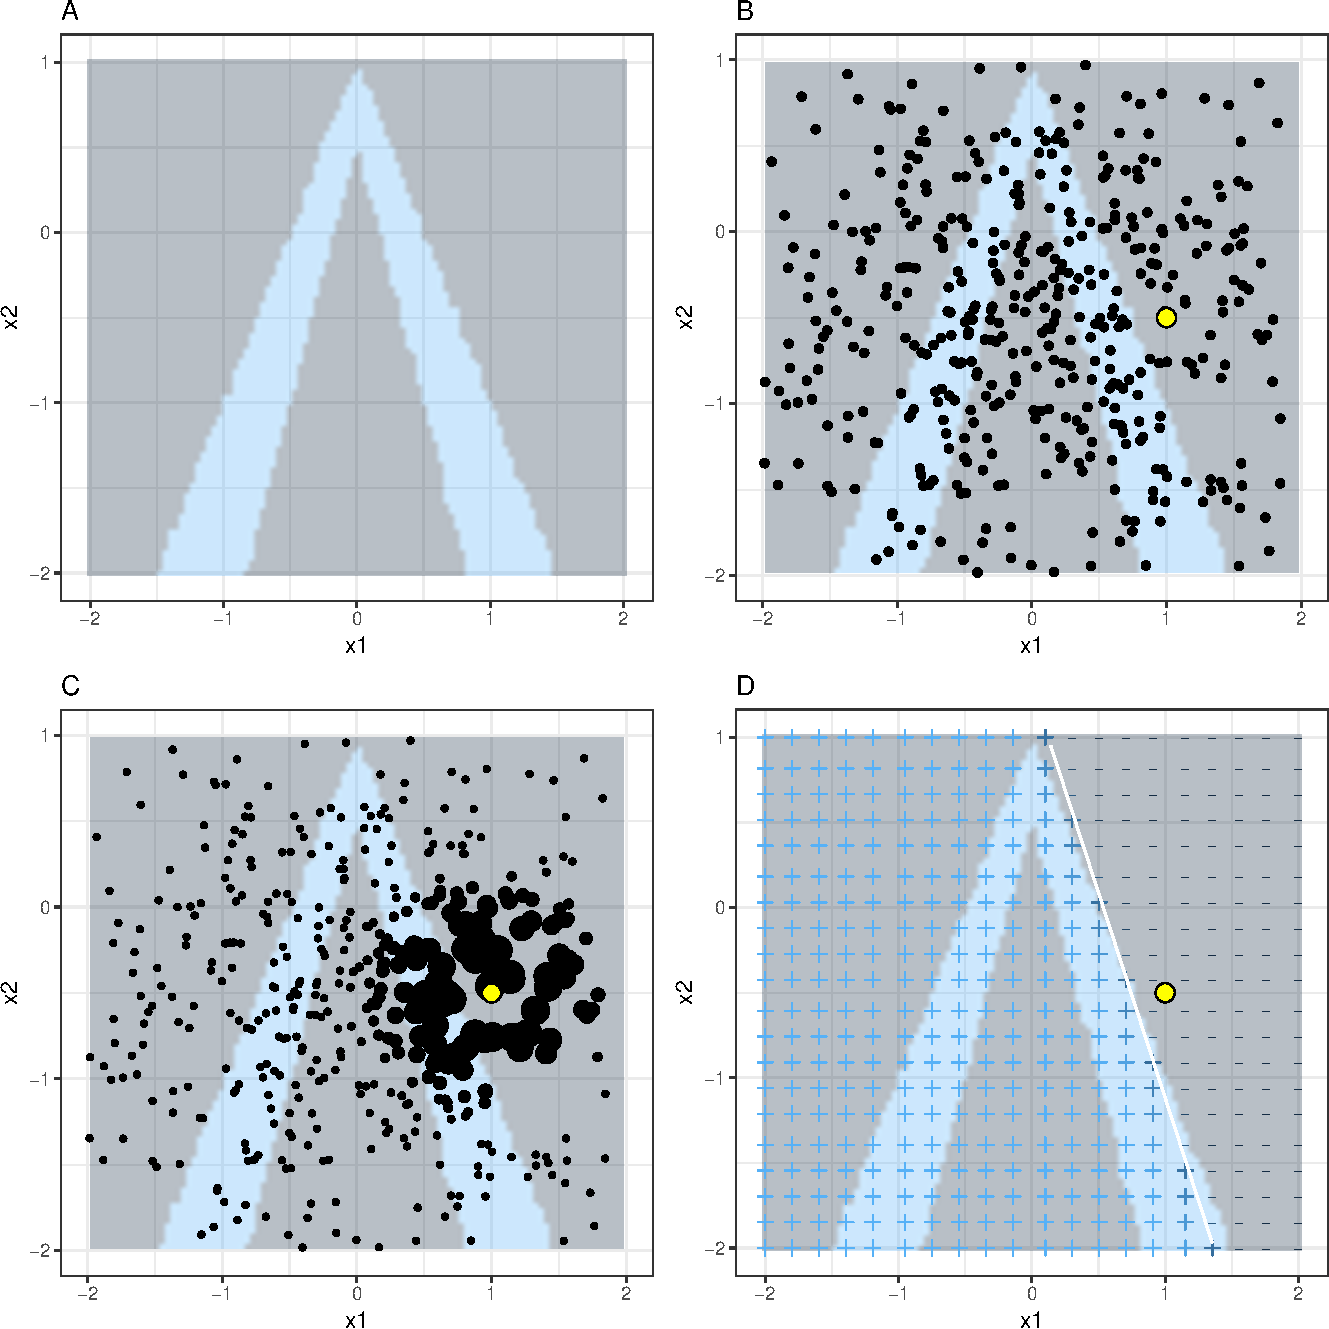
\includegraphics{xai-book_files/figure-latex/lime-fitting-1.pdf}
\caption{\label{fig:lime-fitting}How LIME sampling works: A) The trainig
data has two classes. The most data points have class 0, and the ones
with class 1 are grouped in an upside-down V-shape. The plot displays
the decision boundaries learned by a machine learning model. In this
case it was a Random Forest, but it does not matter, because LIME is
model-agnostic and we only care about the decision boundaries. B) The
yellow is the instance of interest, for which an explanation is desired.
The black dots are data sampled from a normal distribution around the
means of the features in the training sample. This has only to be done
once and can be reused for other explanations. C) Introducing locality
by giving points near the instance of interest a higher weights. D) The
colors and signs of the grid display the classifications of the locally
learned model form the weighted samples. The white line marks the
decision boundary (P(class) = 0.5) at which the classification changes.}
\end{figure}

\subsubsection{Example}\label{example-3}

Let's look at a concrete example. We go back to the bike rental and turn
the prediction problem into a classification: After accounting for the
trend that the bike rental get's more popular over time we want to know
on a given day if the number of rented bikes will be above or below the
trend line. You can also interpret `above' as being above the mean bike
counts, but adjusted for the trend.

First we train a Random Forest on the classification task. Given
seasonal and wheather information, on which day will the number of bike
rentals be above the trend-free average? The Random Forest has 100
trees.
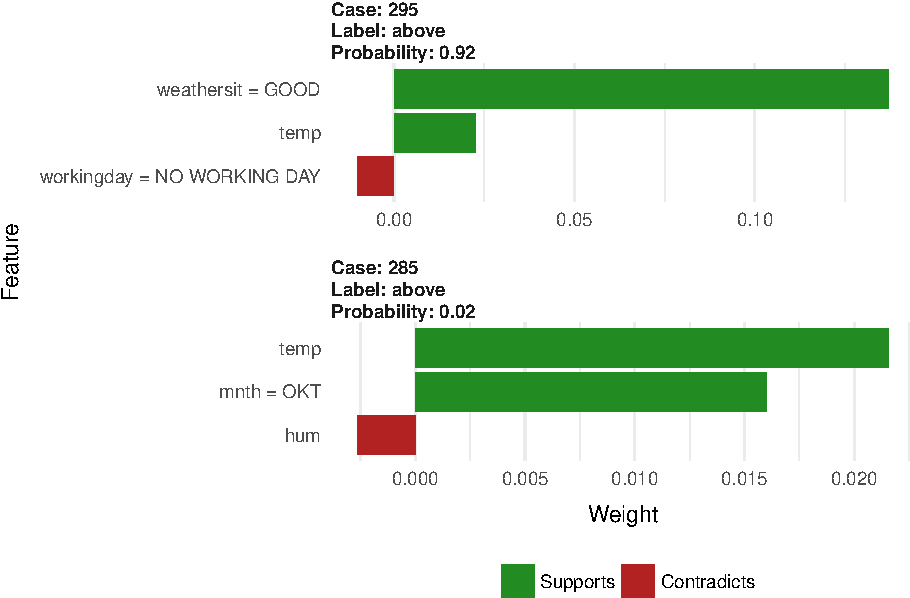
\includegraphics{xai-book_files/figure-latex/lime-tabular-example-explain-plot-1-1.pdf}
The continuous features are categorised into bins by quantiles for the
explanation models. The explanations are set to contain 3 features.
Figure @ref\{fig:lime-tabular-example-explain-plot-1\} shows the results
of the sparse local linear model that was fitted for two instances with
different predicted classes. It becomes clear from the figure, that it
is easier to interpret categorical features than continuous features.
Figure @ref\{fig:lime-tabular-example-explain-plot-2\} shows a variant
where the continuous features are turned into categorial features by
putting them into bins along the quantiles.

\begin{figure}
\centering
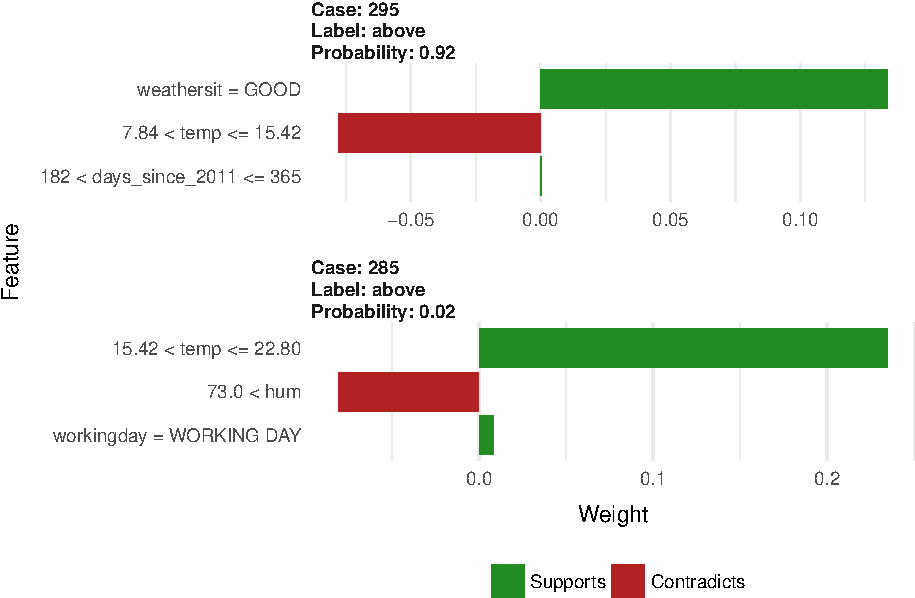
\includegraphics{xai-book_files/figure-latex/lime-tabular-example-explain-plot-2-1.pdf}
\caption{\label{fig:lime-tabular-example-explain-plot-2}Explanations for two
instances. This time continuous features were turned into categorial
features by binning them.}
\end{figure}

\subsubsection{LIME for images}\label{lime-for-images}

For images the sampling procedure works differently. Instead of sampling
single pixels, LIME create variations of the image by turning off
superpixel.

\subsubsection{LIME for text}\label{lime-for-text}

LIME for text works a bit differently than for tabular data. Variation
of the point to be explained are created differently: Starting from the
original text, new texts are created by randomly removing words from it.

\subsubsection{Example}\label{example-4}

In this example we classify spam vs.~ham of YouTube comments. The
dataset is described in {[}\#TubeSpam{]}.

The black box model is a decision tree on the document word matrix. Each
comment is one document (= one row) and each column is a the number of
occurences of a specific word. A decision tree was trained on this data.
As discussed in Section {[}\#simple{]}, decision trees are easy to
understand, but in this case the tree is very deep. Also in the place of
this tree there could have been a recurrent neural network or a support
vector machine that was trained on the embeddings from word2vec. The
machine learning model was trained on 80\% of the approximately 2000
comments. From the remaining comments two were selected for showing the
explanations.

Let's look at tow comments of this dataset and the corresponding
classes:

\hypertarget{htmlwidget-a7e2e3f97b18ee50788e}{}

In the next step we create some variations of the datasets, which are
used in a local model. For example some variations of one of the
comments.

\hypertarget{htmlwidget-d2a25d7a243dd7d0fdba}{}

Each column corresponds to one word in the sentence. Each row is a
variation. 1 indicates that the word is part of this variation. 0
indicates that the word was removed. The corresponding sentence for the
first variation is ``\texttt{Guy\ in\ the\ yellow\ suit\ Jae-suk}''.

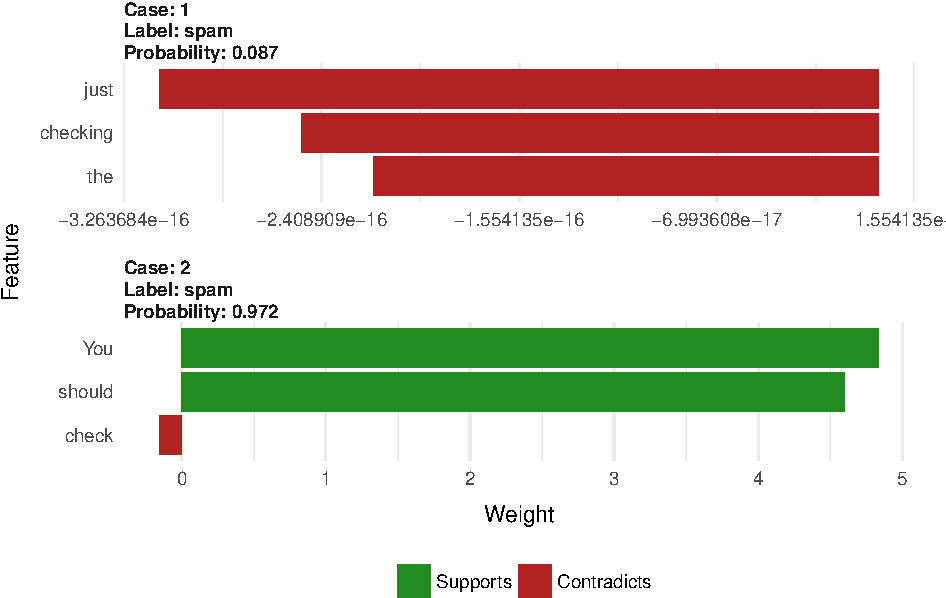
\includegraphics{xai-book_files/figure-latex/lime-text-explanations-1.pdf}
\#\#\#\# Problems with LIME

\begin{itemize}
\tightlist
\item
  LIME does not work if the classification is very unbalanced (one class
  is very common) and the black box only predicts one class
\item
  Defining the neighbourhood is tricky.
\end{itemize}

\bibliography{book.bib}

\backmatter
%\printindex


\end{document}
